\chapter{Physics Analysis}
%================================================================

This chapter will discuss about the cross section measurement of the associated production of $\Upsilon$ and $D^{*\pm}$ using the full CMS Run 2 data with 13 TeV center-of-mass energy. \textcolor{red}{falar mais}

\section{Datasets and Simulation}
\subsection{Data Samples}

The data samples were recorded by the CMS detector during the LHC Run 2 in 2016-2018 at a center-of-mass energy of 13 TeV and are composed only by events certified as good for physics analysis. The Table \ref{tab:datasamples} displays all the data samples used. The total recorded luminosity of all data samples is 137.61 fb$^{-1}$.

\begin{table}[!htbp]{15cm}
  \caption{Data samples considered in this work}\label{tab:datasamples}
  \begin{tabular}{ c }
    Dataset \\ 
    \hline
    /MuOnia/Run2016B-21Feb2020\_ver1\_UL2016\_HIPM-v1/AOD \\
    /MuOnia/Run2016B-21Feb2020\_ver2\_UL2016\_HIPM-v1/AOD \\
    /MuOnia/Run2016C-21Feb2020\_UL2016\_HIPM-v1/AOD \\
    /MuOnia/Run2016D-21Feb2020\_UL2016\_HIPM-v1/AOD \\
    /MuOnia/Run2016E-21Feb2020\_UL2016\_HIPM-v1/AOD \\
    /MuOnia/Run2016F-21Feb2020\_UL2016\_HIPM-v1/AOD \\
    \hline
    /MuOnia/Run2016F-21Feb2020\_UL2016-v1/AOD \\
    /MuOnia/Run2016G-21Feb2020\_UL2016-v1/AOD \\
    /MuOnia/Run2016H-21Feb2020\_UL2016-v1/AOD \\
    \hline
    /MuOnia/Run2017B-09Aug2019\_UL2017-v1/AOD \\
    /MuOnia/Run2017C-09Aug2019\_UL2017-v1/AOD \\
    /MuOnia/Run2017D-09Aug2019\_UL2017-v1/AOD \\
    /MuOnia/Run2017E-09Aug2019\_UL2017-v1/AOD \\
    /MuOnia/Run2017F-09Aug2019\_UL2017-v1/AOD \\
    \hline
    /MuOnia/Run2018A-12Nov2019\_UL2018-v1/AOD \\
    /MuOnia/Run2018B-12Nov2019\_UL2018-v1/AOD \\
    /MuOnia/Run2018C-12Nov2019\_UL2018-v1/AOD \\
    /MuOnia/Run2018D-12Nov2019\_UL2018-v1/AOD \\
  \end{tabular}
  \legend{Data Samples used in the analysis corresponding to the full CMS Run 2 data taking.}
\end{table}

From the analysis point view, data samples are divided into four subsamples (2016APV, 2016, 2017 and 2018), to take into account the differences in the detector in the course of Run 2 (e.g. lose in the efficiency due to aging and installation of new detectors).

\subsection{Simulation Samples}

The simulation samples are done via Monte Carlo (MC) simulation, where the MC method is used in programs to model the physics processes. The starting point of the simulation is the event generation, where the events following a set of physics processes of interest are created by the MC generator.

First, the parton level matrix element of the process is calculated perturbatively up to a fixed order. After, the parton showering is done to take into account the higher order effects, such as initial and final state radiation (ISR and FSR). This is followed by the hadronization, where the quarks and gluons form the quarks. Finally, the simulation should also handle the particles decay.

The detector simulation follows the event generation. Here, the interaction of the generated particles with the detector is simulated. In CMS, the detector response is simulated using \textsc{Geant4} \cite{GEANT4:2002zbu}. The simulated detector response pass through the same processing chain as the real data forming the final simulated sample.

The MC samples were used in this analysis to simulate the two components of the signal, the SPS and DPS. The only background was not simulated, since it is only combinatorial

The DPS was created using the \textsc{Pythia8} \cite{Sjostrand:2014zea} as event generator, parton showering and for hadronization. For the decays of the heavy flavour hadrons, \textsc{EvtGen} \cite{Lange:2001uf} was used. The SPS sample is similar to the DPS, with the addition of the \textsc{HELAC-Onia} \cite{Shao:2012iz, Shao:2015vga}, which was used for event generation.

In the same way as the data, the MC samples are divided into subsamples to take into account the detector differences in the course of Run 2. The detector simulation is tunned to better represent the detector conditions in each subsample.

\textcolor{red}{colocar imagens da simulação}

\section{\texorpdfstring{$\Upsilon$ + D$^{*\pm}$}{Y+D*} Reconstruction}

The $\Upsilon$ + D$^*$ reconstruction is done from the reconstructed tracks in an event. As shown in Fig. \ref{fig:drawing_event}, there are five different particles in the final state an event - three coming from D$^*$ and two from $\Upsilon$. The D$^*$ have a low combinatorial background when compared with other open charm mesons because of it very characteristic signature - very small difference of mass between D$^*$ and D$^0$ restricting the phase space of the slow pion. Also, the kaon and pion can be identified even without a particle identification detector, since it should have a opposite charge to the slow pion, removing the ambiguity of the D$^0$ reconstruction.

\begin{figure}[!htm]{15cm}
\caption{Drawing of an event of associated production of $\Upsilon$ and D$^{*+}$}%
\label{fig:drawing_event}
\fbox{
\begin{tikzpicture}
  \coordinate (PV) at ( 0,0);
  \coordinate (SV) at ( 2.0,1.8);
  \coordinate (BL) at (-3,0);
  \coordinate (BR) at ( 4,0);

  \draw[beamcol,dashed,name path=beam]
    (BL) -- (BR);
  \draw[SVcol,dashed]
    (PV) -- (SV)
    node[midway,above=0.1,left=0.1] {$D^0$};

  \draw[->,mygreen,line width=1]
    (SV) to[bend right] (1.0,3.0) node[above right] {$\pi^+$};
  \draw[->,mygreen,line width=1]
    (SV) to[bend left] (3.0,3.0) node[above left] {$K^-$};

  \draw[->,red,line width=1]
    (PV) to[bend right=20] (-2.0,1.0) node[below right] {$\mu^+$};
  \draw[->,red,line width=1]
    (PV) to[bend left=20] (-1.0,2.0) node[below left] {$\mu^-$};


  \draw[->,SVcol,line width=1]
    (PV) arc[start angle=150, end angle=0, radius=0.5] node[below right] {$\pi_s^+$};
  
  \fill[beamcol]
    (PV) ellipse (9pt and 4.5pt)
    node[beamcol!95!black,below left] {PV $\color{red}{\Upsilon} \color{beamcol}{+} \color{SVcol}{D^*}$};
  \fill[SVcol]
    (SV) circle (4pt) node[below right] {SV};
\end{tikzpicture}
}
\legend{Drawing of an event of associated production of $\Upsilon$ and D$^*$. $\Upsilon$ decays into two opposite charge muons, while D$^{*+}$ decays into a pion and D$^0$, which later decays into a kaon and a pion.}
\end{figure}

The D$^*$ reconstruction starts by finding a suitable D$^0$ candidate. For this, two tracks of opposite charge are paired to check whether they form a common vertex using the Kalman Filter method \cite{Fruhwirth:1991pm, Speer:927395}. If the fit is valid and its p-value is greater than 1\%, the D$^0$ candidate is selected. The vertex determination also allows for a better calculation of the kinematic variables of the tracks and it is called secondary vertex (SV).

A primary vertex (PV) is assigned to the D$^0$ candidate as the one closest to the SV in order to calculate the decay length, defined as
\begin{equation}
    dl = \frac{|\Vec{p}_{D^0} \cdot \Delta\Vec{l}|}{|\Vec{p}_{D^0}|},
\end{equation}
where $\Vec{p}_{D^0}$ is the D$^0$ trimomentum and $\Delta\Vec{l}$ is the distance between the PV and SV, the decay length significance is very important because it can be used to filter a lot of background, it is defined as
\begin{equation}
    dl_{sig} = \frac{dl}{dl_{err}},
\end{equation}
where $dl_{err}$ is the uncertainty of $dl$. Finally, another important variable is the cosine of the angle between the PV and SV position vectors (pointing angle)
\begin{equation}
    \cos{\alpha} = \frac{dl}{\Delta\Vec{l}} \; ,
\end{equation}
which hints the alignment between the PV and the SV.

After the D$^0$ candidates is reconstructed, a new track coming from the same PV of the D$^0$ is added to form the D$^*$ candidate and its momentum resolution is improved by adding the PV to the track fit.

The $\Upsilon(nS)$ reconstruction is done in a similar way to the D$^0$. Two muons with opposite charge are selected and its vertex is determined from the fit. If the vertex is valid and has a p-value greater than 1\% we have a dimuon candidate. The invariant mass of the dimuon should be in the range of $8.5 < m_{\mu\mu} < 11.5$ GeV in order to be classified as a $\Upsilon(nS)$ candidate. 

Finally, in order to pair the $\Upsilon(nS)$ and the $D^*$, a vertex fit of the two muons and the slow pion is performed. If valid, the vertex p-value is determined.

In this stage of the reconstruction, very loose cuts are applied to the candidates, those are specified in the Sec. \ref{subsec:preselcuts}.

\section{Event Selection}\label{sec:evtsel}

\subsection{Preselection Cuts} \label{subsec:preselcuts}

Preselection cuts are used to mitigate some of the combinatorial background and save disk space when recording the NTuple. They are very loose and are further improved when the analysis final cuts are applied (Sec. \ref{sec:selcuts}). The preselection cuts both for the $\Upsilon$ and the D$^*$ candidates are summarized in the Tab. \ref{tab:preselectioncuts}.

\begin{table}[!htbp]{15cm}
  \caption{Preselection cuts.}
  \begin{tabular}{ l | l }
    \hline
    \multicolumn{1}{c|}{Variable} & \multicolumn{1}{|c}{Cut} \\ \hline
    \multicolumn{2}{c}{D$^*$ candidate} \\ \hline
    Transverse momentum of $K$ and $\pi$ ($p_T^{K, \pi}$) & $> 0.3$ GeV \\ \hline
    Transverse and longitudinal impact parameter & \multirow[c]{2}{*}{$< 0.5$ cm} \\ 
    of $K$ and $\pi$ track ($d_{xy}$ and $d_z$) & \\ \hline
    Transverse and longitudinal impact parameter & \multirow[c]{2}{*}{$< 2$ cm} \\ 
    of $\pi_s$ track ($d_{xy}$ and $d_z$) & \\ \hline
    Longitudinal distance between D$^0$ vertex and PV & $< 2$ cm \\ \hline
    Transverse momentum of D$^0$ ($p_T^{D^0}$) & $> 0.9$ GeV \\ \hline
    D$^0$ of D$^{*\pm}$ mass cut ($m_{D^0}$) & $1.5 < m_{D^0} < 2.3$ GeV \\ \hline
    Mass difference between D$^{*\pm}$ and D$^0$ ($\Delta m$) & $< 0.17$ GeV \\ \hline
    $D^0$ candidate vertex probability & $> 0.01$ \\ \hline

    \multicolumn{2}{c}{$\Upsilon$ candidate} \\ \hline
    Pseudorapidity separation between the two $\mu$ ($\Delta\eta_{\mu^+\mu^-}$) & $< 3.0$ \\ \hline
    Transverse and longitudinal impact parameter & \multirow[c]{2}{*}{$< 0.5$ cm} \\ 
    of the two $\mu$ tracks & \\ \hline
    Longitudinal distance between the dimuon & \multirow[c]{2}{*}{$< 0.5$ cm} \\ 
    candidate vertex and the PV & \\ \hline
    Dimuon candidate vertex probability & $> 0.01$ \\ \hline
    Dimuon mass range & $8.5 < m_{\mu\mu} < 11.5$ GeV \\ \hline
  \end{tabular}
  \legend{Preselection cuts used to save disk space when saving the NTuples.}
  \label{tab:preselectioncuts}
\end{table}

\textcolor{red}{colocar imagens da pre seleção?}

\subsection{Trigger}\label{sec:trigger}

The trigger strategy chosen was to use the HLT Paths that filters dimuons, it was required that the trigger had the maximum possible rapidity coverage, to use for discrimination between DPS and SPS, and lower $p_T$ threshold. The used trigger paths are specified in Tab. \ref{tab:triggers} all of them required two muons with opposite charge, invariant mass between 8.5 and 11.5 GeV, reconstructed pseudorapidity < 2.5 and are unprescaled. In addition to those, there is a cut in transverse momentum different for each trigger path.

In the year 2017, the chosen trigger was not available in the whole data-taking resulting in a lower recorded luminosity (the total was 41.48 fb$^{-1}$ in full 2017 data). This should not pose a problem, since the statistics are large (123.1 fb$^{-1}$ for the three years) and the other triggers did only cover the central area of the detector, which can turn the discrimination between SPS and DPS more complicated. 

\begin{table}[!htbp]{15cm}
  \caption{Triggers used in this study in each year of data taking}
  \begin{tabular}{ c | c | c | c | c }
    Year & Trigger Path & $p_T$ Cut (GeV) & Recorded L ($fb^{-1}$) & L Uncertainty \\  \hline
    \multirow[c]{2}{*}{2016} & HLT\_Dimuon13 & \multirow[c]{2}{*}{$>12.9$} & \multirow[c]{2}{*}{36.18} & \multirow[c]{2}{*}{2.5 \%} \\
    & \_Upsilon & & \\ \hline
    \multirow[c]{2}{*}{2017} & HLT\_Dimuon24 & \multirow[c]{2}{*}{$>13.9$} & \multirow[c]{2}{*}{27.12} & \multirow[c]{2}{*}{2.3 \%} \\ 
    & \_Upsilon\_noCorrL1 & & & \\ \hline
    \multirow[c]{2}{*}{2018} & HLT\_Dimuon24 & \multirow[c]{2}{*}{$>13.9$} & \multirow[c]{2}{*}{59.82} & \multirow[c]{2}{*}{2.5 \%} \\
    & \_Upsilon\_noCorrL1 & & & \\ \hline
  \end{tabular}
  \legend{Triggers used in this study in each year of data taking. The luminosity uncertainty for each year can be found in \cite{CMS-PAS-LUM-17-001, CMS-PAS-LUM-17-004, CMS-PAS-LUM-18-002}}
  \label{tab:triggers}
\end{table}

\subsection{Selection Cuts} \label{sec:selcuts}

The analysis cuts are tighter cuts applied to the data in order to define the fiducial volume and to improve the signal to background ratio. A summary of them are displayed in the Tabs. \ref{tab:fiducialvol} and \ref{tab:selectioncuts}.

\begin{table}[!htbp]{15cm}
  \caption{Kinematic cuts that define the fiducial volume.}
  \begin{tabular}{ l | l }
    \hline
    \multicolumn{1}{c|}{Variable} & \multicolumn{1}{|c}{Cut} \\ \hline
    $\mu$ transverse momentum ($p_T^\mu$) & $> 3$ GeV \\ \hline
    $\mu$ pseudorapidity ($\eta_\mu$) & $|\eta_\mu| < 2.4$ \\ \hline
    $\Upsilon$ transverse momentum ($p_T^\Upsilon$) & $15 < p_T^\Upsilon < 150$ GeV \\ \hline
    $\Upsilon$ rapidity ($y_\Upsilon$) & $|y_\Upsilon| < 2.5$ \\ \hline
    Transverse momentum of $K$ and $\pi$ ($p_T^{K, \pi}$) & $> 1$ GeV \\ \hline
    Transverse momentum of $\pi_s$ ($p_T^{\pi_s}$) & $> 0.3$ GeV \\ \hline
    Transverse momentum of D$^0$ ($p_T^{D^0}$) & $> 3$ GeV\\ \hline
    D$^*$ transverse momentum ($p_T^{D^*}$) & $4 < p_T^{D^*} < 80$ GeV \\ \hline
    D$^*$ rapidity ($y_{D^*}$) & $|y_{D^*}| < 2.5$ \\ \hline
  \end{tabular}
  \legend{Cuts on the kinematic variables of the system that define the fiducial volume of the analysis.}
  \label{tab:fiducialvol}
\end{table}

\begin{table}[!htbp]{15cm}
  \caption{Selection cuts.}
  \begin{tabular}{ l | l }
    \hline
    \multicolumn{1}{c|}{Variable} & \multicolumn{1}{|c}{Cut} \\ \hline
    \multicolumn{2}{c}{D$^*$ candidate} \\ \hline
    Track $\chi^2$ of $K$ and $\pi$ & $< 2.5$ \\ \hline
    Number of valid tracker detector hits for $K$ and $\pi$ & $> 4$ \\ \hline
    Number of valid pixel detector hits for $K$ and $\pi$ & $> 1$ \\ \hline
    transverse impact parameter of $K$ and $\pi$ from PV & 0.5 cm \\ \hline
    longitudinal impact parameter of $K$ and $\pi$ & \multirow[c]{2}{*}{0.5/$\sin{\theta}$ cm} \\
    from PV & \\ \hline
    Track $\chi^2$ of $\pi_s$ & $< 3$ \\ \hline
    Number of valid tracker detector hits for $\pi_s$ & $> 2$\\ \hline
    D$^0$ mass ($m_{D^0}$) & $|m_{D^0} - 1.864| < 0.028$ GeV \\ \hline
    D$^0$ cosine of the pointing angle ($\cos{\alpha_{D^0}}$) & $> 0.99$ \\ \hline
    D$^0$ decay length significance ($dl_{sig}$) & $> 2.7$ \\ \hline
    
    \multicolumn{2}{c}{$\Upsilon$ candidate} \\ \hline
    $\mu$ soft id flag & soft id = True \\ \hline

    \multicolumn{2}{c}{$\Upsilon$ + D$^*$ candidate} \\ \hline
    $\mu\mu\pi_s$ vertex probability & $> 0.01$ \\ \hline

  \end{tabular}
  \legend{Selection cuts used to improve the signal to background ratio.}
  \label{tab:selectioncuts}
\end{table}

The cuts on Tab. \ref{tab:fiducialvol} were based on studies using MC simulations on the expected acceptance of the detector to each one of the objects. The cuts on the slow pion are more loose to the other tracks, in special, the transverse momentum cut is very important, as it directly correlated to the lower limit of the D$^*$ transverse momentum, since the slow pion phase space is restricted by the low mass difference between D$^0$ and D$^*$. Also, the cut on the D$^0$ observables listed in Tab. \ref{tab:selectioncuts} are very important to improve the D$^*$ signal to background ratio at the expense to reduce greatly the statistics of the sample, so they were very well tunned for this work. 

On Tab. \ref{tab:selectioncuts} the soft id flag refers to the following selections on the muon: 
\begin{itemize}
  \item Muon track in tracker detector matched with at least one segment in the muon detector (in any station) in both X and Y coordinates (< 3$\sigma$).
  \item Number of tracker layers with hits > 5, to guarantee good $p_T$ measurement. 
  \item Number of pixel layers > 0.
  \item Muon track has high-purity flag, rejecting bad quality tracks
  \item Transverse and longitudinal impact parameter cuts, dxy < 0.3 cm and dz < 20 cm w.r.t. the primary vertex.
\end{itemize}

\textcolor{red}{colocar imagens da seleção}

\section{Signal Extraction}\label{sec:sig_extraction}

The signal extraction is performed by doing a 2D fit to the dimuon invariant mass ($m_{\mu\mu}$) and D$^*$ $\Delta m$ distributions. To fulfill this a description of the signal and background for each distribution is created and a product of both is taken as the 2D model. Each of the distribution models contains components for signal and background and a non-extended composite PDF is constructed. The fit is performed using the RooFit package.

\subsection{\texorpdfstring{$\Upsilon$}{Y} Model}

The fit model has three signal components, one for each of the observed $\Upsilon(nS)$ states. All of them are modeled using the Crystal Ball distribution, defined as
\begin{equation}
  CB(x;\alpha,n,\bar x,\sigma) = N \cdot 
  \begin{cases} 
    \exp(- \frac{(x - \bar x)^2}{2 \sigma^2}), & \mbox{for }\frac{x - \bar x}{\sigma} > -\alpha \\
    A \cdot (B - \frac{x - \bar x}{\sigma})^{-n}, & \mbox{for }\frac{x - \bar x}{\sigma} \leqslant -\alpha 
  \end{cases}
\end{equation}
where
\begin{equation}
\begin{split}
  A = & \left(\frac{n}{\left| \alpha \right|}\right)^n \cdot \exp\left(- \frac {\left| \alpha \right|^2}{2}\right), \\
  B = & \frac{n}{\left| \alpha \right|}  - \left| \alpha \right|, \\
  N = & \frac{1}{\sigma (C + D)}, \\
  C = & \frac{n}{\left| \alpha \right|} \cdot \frac{1}{n-1} \cdot \exp\left(- \frac {\left| \alpha \right|^2}{2}\right), \\
  D = & \sqrt{\frac{\pi}{2}} \left(1 + \operatorname{erf}\left(\frac{\left| \alpha \right|}{\sqrt 2}\right)\right). \\
\end{split}
\end{equation}
With N as the normalization factor, $\alpha$, $n$, $\bar x$ and $\sigma$ are the fit parameters and erf is the error function. This function behaves like a Gaussian for $(x-\bar x)/\sigma$ greater than $-\alpha$ and presents a tail for values less than equals $-\alpha$, being able to model the effects of FSR to the dimuon invariant mass distribution.

In order to reduce the amount of free parameters of the fit, the following constraints are imposed to the CB parameters:
\begin{itemize}
  \item The mean of all the CBs are fixed to the PDG mass value of its $\Upsilon$ state times a mass scale (to take into account the uncertainties on muon momentum scale calibration). $\bar x_{\Upsilon(nS)} = m_{scale}\cdot m_{\Upsilon(nS)}$;
  \item The sigma of the CBs used to model 2S and 3S states are set to be proportional to their mass ratio with respect to the 1S state. Therefore, only one sigma is taken as free parameter. $\sigma_{\Upsilon(2S)} = \sigma_{1S}\times m_{\Upsilon(2S)}/m_{\Upsilon(1S)}$ and $\sigma_{\Upsilon(3S)} = \sigma_{1S}\times m_{\Upsilon(3S)}/m_{\Upsilon(1S)}$;
  \item The tail parameters ($\alpha$ and $n$) are set as the same for the three CBs;
\end{itemize}

Finally, the fit model for $\Upsilon(nS)$ signal is
\begin{equation} \label{eq:upsilon_sig}
  S_{\Upsilon}(m_{\mu\mu}) = f_{\Upsilon(1S)}\cdot CB_{\Upsilon(1S)} (m_{\mu\mu}) + f_{\Upsilon(2S)}\cdot CB_{\Upsilon(2S)} (m_{\mu\mu}) + (1-f_{\Upsilon(1S)}-f_{\Upsilon(2S)}) \cdot CB_{\Upsilon(3S)} (m_{\mu\mu})
\end{equation}

For the background, Chebychev polynomials of the first kind are used up to second order. They are defined as:
\begin{equation} \label{eq:upsilon_bkg}
\begin{split}
  T_0(x) = & 1 \\
  T_1(x) = & x \\
  T_{n+1}(x) = & 2xT_n(x) - T_{n-1}(x).
\end{split}
\end{equation}
The background component is written as
\begin{equation}
  B_{\Upsilon}(m_{\mu\mu}) = N[1 + b_1 T_1(m_{\mu\mu}) + b_2 T_2(m_{\mu\mu})],
\end{equation}
where N is the normalization constant and $b_1$ and $b_2$ as free parameters for the fit.

The 1D fit to the 2018 data sample is given in Fig. \ref{fig:fit1D_upsilon}.

\begin{figure}[!htm]{15cm}
  \caption{One dimensional fit to selected $\Upsilon$ data}%
  \label{fig:fit1D_upsilon}
  \fbox{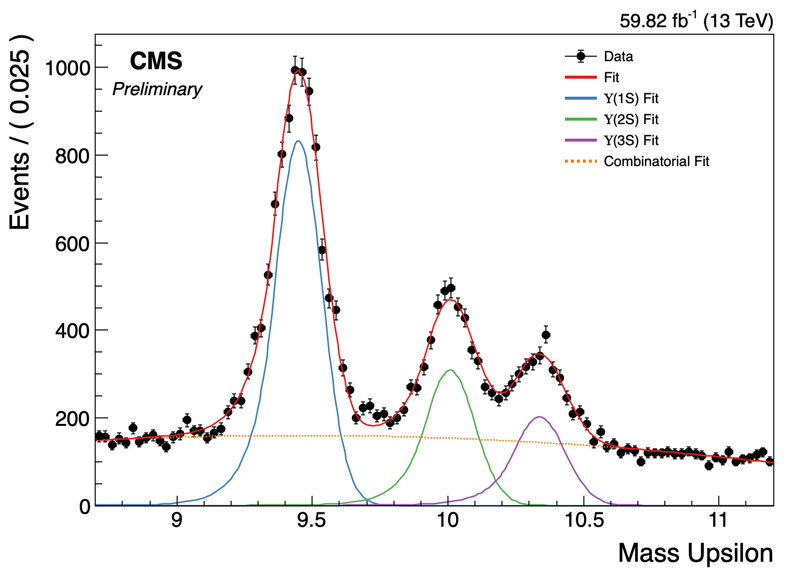
\includegraphics[width=0.68\textwidth]{figures/fit/upsilon_2018_fit.png}}
  \legend{One dimensional fit to selected $\Upsilon$ 2018 data sample. The fit is done to separate signal from the background for the three $\Upsilon$ states. The curves represent the fit for the full model (red) and each of the components (blue, green and purple for the $\Upsilon(1S)$, $\Upsilon(2S)$ and $\Upsilon(3S)$ signal and dashed orange for the combinatorial background).}
\end{figure}

\subsection{\texorpdfstring{D$^{*}$}{D*} Model}

For D$^*$ signal component, it is used a Johnson's distribution
\begin{equation}\label{eq:dstar_sig}
  S_{D^*}(\Delta m) = \frac{\delta}{\lambda\sqrt{2\pi}} \frac{1}{\sqrt{1 + \left(\frac{\Delta m-\mu}{\lambda}\right)^2}}\exp{\left[-\frac{1}{2}\left(\gamma+\delta\sinh^{-1}\left(\frac{\Delta m-\mu}{\lambda}\right)\right)^2\right]},
\end{equation}
where $\delta$, $\lambda$, $\gamma$ and $\mu$ are the free parameters. This function is often used to describe the mass difference of charm decays and fits well the $\Delta$m distribution.

For the D$^*$ background, a threshold function \cite{ZEUS:2013fws} given by:
\begin{equation} \label{eq:dstar_bkg}
  B_{D^*}(\Delta m) = A \cdot (\Delta m - m_\pi)^B \cdot \exp[C\cdot (\Delta m-m_\pi)]
\end{equation}
is used, where $m_\pi$ is the pion mass and $A$, $B$ and $C$ are free parameters.

The 1D fit to the 2018 data sample is given in Fig. \ref{fig:fit1D_dstar}.

\begin{figure}[!htm]{15cm}
  \caption{One dimensional fit to the selected D$^{*\pm}$ data}%
  \label{fig:fit1D_dstar}
  \fbox{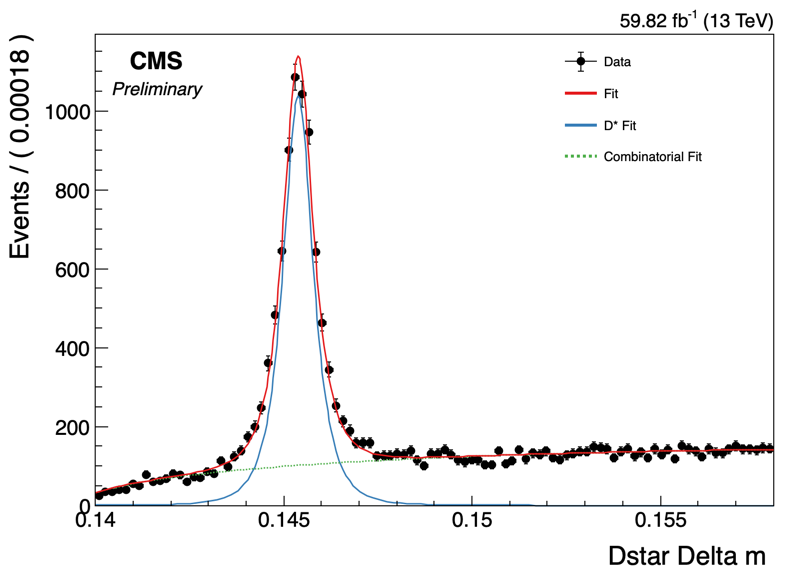
\includegraphics[width=0.68\textwidth]{figures/fit/dstar_2018_fit.png}}
  \legend{One dimensional fit to the selected D$^{*\pm}$ 2018 data sample. The curves represent the fit for the full model (red) and each of the components (blue for signal and dashed green for the combinatorial background).}
\end{figure}

\subsection{\texorpdfstring{$\Upsilon$ + D$^{*}$}{Y+D*} 2D Model}

Finally, the construction of the 2D model takes into account the 4 distributions from Eqs. \ref{eq:upsilon_sig}, \ref{eq:upsilon_bkg}, \ref{eq:dstar_sig} and \ref{eq:dstar_bkg}, creating the final four component distribution:
\begin{equation}
\begin{split}
  M_{\Upsilon D^*}(m_{\mu\mu}, \Delta m) & = f_s \cdot S_\Upsilon(m_{\mu\mu}) \cdot S_{D^*}(\Delta m) \\
  & + f_{b1} \cdot S_\Upsilon(m_{\mu\mu}) \cdot B_{D^*}(\Delta m) \\
  & + f_{b1} \cdot B_\Upsilon(m_{\mu\mu}) \cdot S_{D^*}(\Delta m) \\ 
  & + (1-f_{b1}-f_{b2}) \cdot B_\Upsilon(m_{\mu\mu}) \cdot B_{D^*}(\Delta m)
\end{split}
\end{equation}

The firs component, composed by both signal models, is used to estimate the associated $\Upsilon$ and D$^*$ yield.

The projections to the dimuon invariant mass and D$^*$ $\Delta$m, extracted from the fit for all data samples, are given in Fig. \ref{fig:fit2D_upsilondstar}.

\begin{landscape}
  \begin{figure}[!htm]{23.7cm}
    \caption{Projections of the two dimensional fit to the selected associated $\Upsilon +$ D$^{*\pm}$ for all data samples.} 
    \label{fig:fit2D_upsilondstar}
    \subfloat[][2016APV $\Upsilon$ projection.]{\label{subfig:fit2D_upsilon_proj_2016APV}%
      \fbox{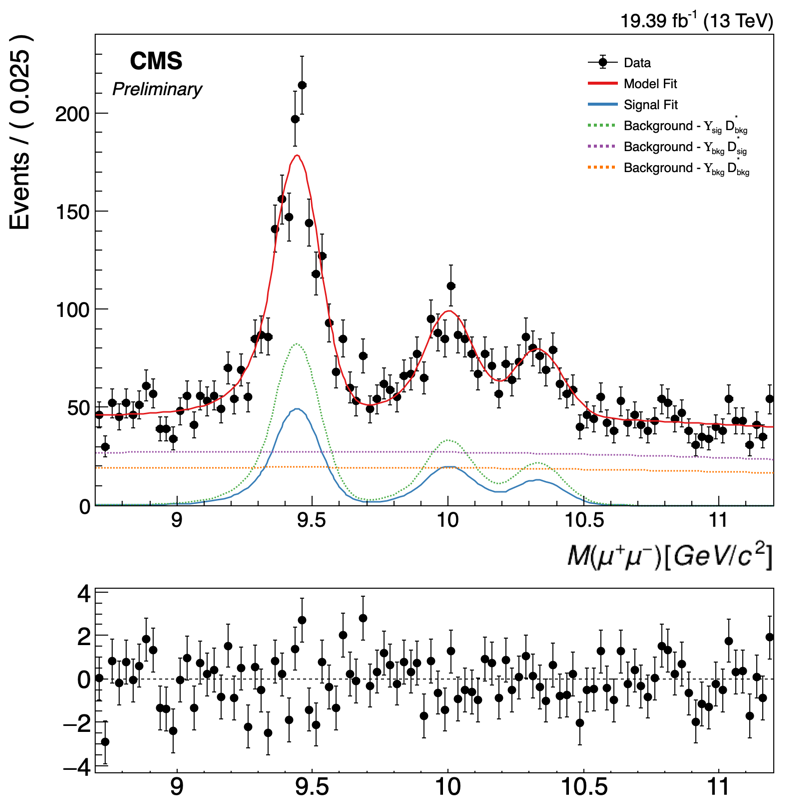
\includegraphics[width=0.23\textwidth]{figures/fit/fit2D_upsilon_proj_2016APV.png}}}\hfill
    \subfloat[][2016 $\Upsilon$ projection.]{\label{subfig:fit2D_upsilon_proj_2016}%
      \fbox{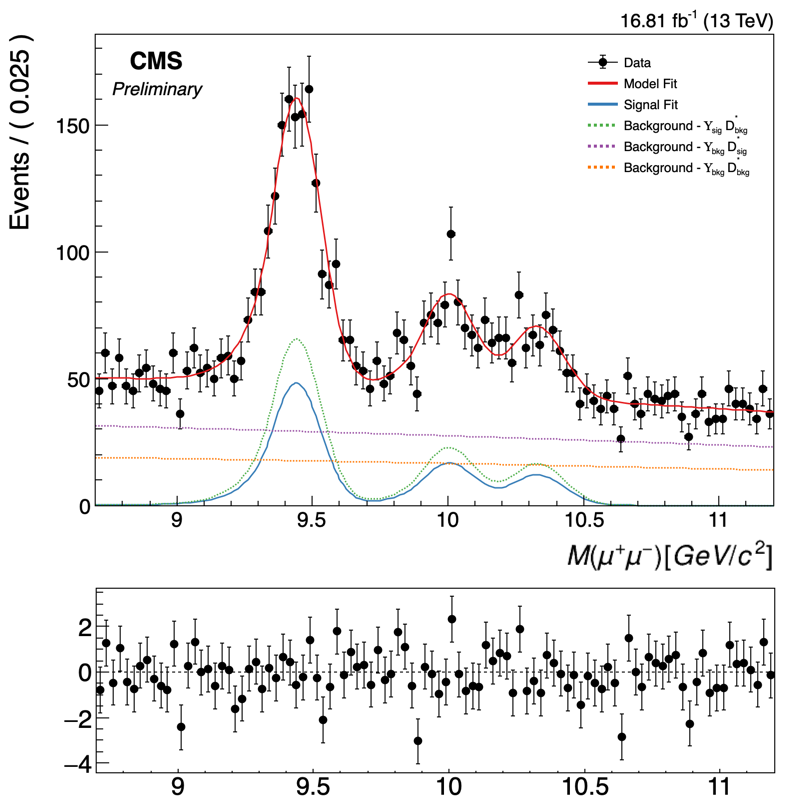
\includegraphics[width=0.23\textwidth]{figures/fit/fit2D_upsilon_proj_2016.png}}}\hfill
    \subfloat[][2017 $\Upsilon$ projection.]{\label{subfig:fit2D_upsilon_proj_2017}%
      \fbox{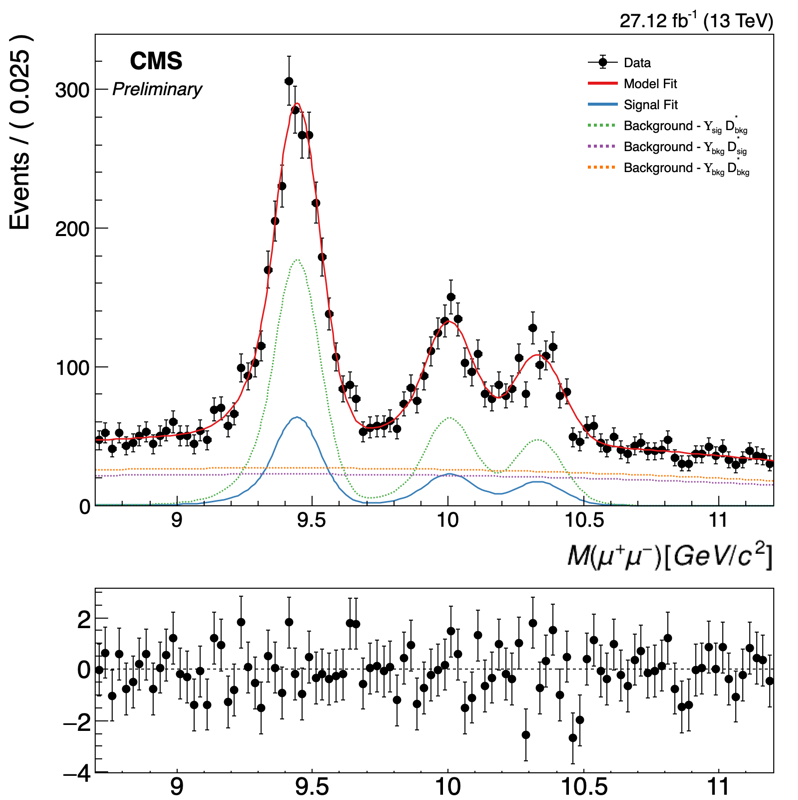
\includegraphics[width=0.23\textwidth]{figures/fit/fit2D_upsilon_proj_2017.png}}}\hfill
    \subfloat[][2018 $\Upsilon$ projection.]{\label{subfig:fit2D_upsilon_proj_2018}%
      \fbox{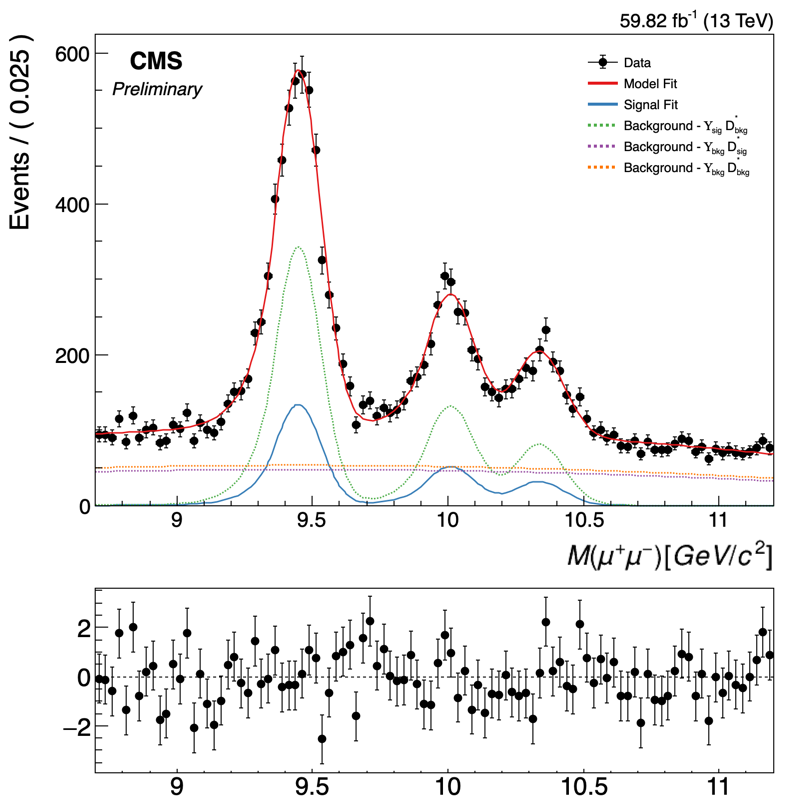
\includegraphics[width=0.23\textwidth]{figures/fit/fit2D_upsilon_proj_2018.png}}}\\
    \subfloat[][2016APV D$^{*\pm}$ projection.]{\label{subfig:fit2D_dstar_proj_2016APV}%
      \fbox{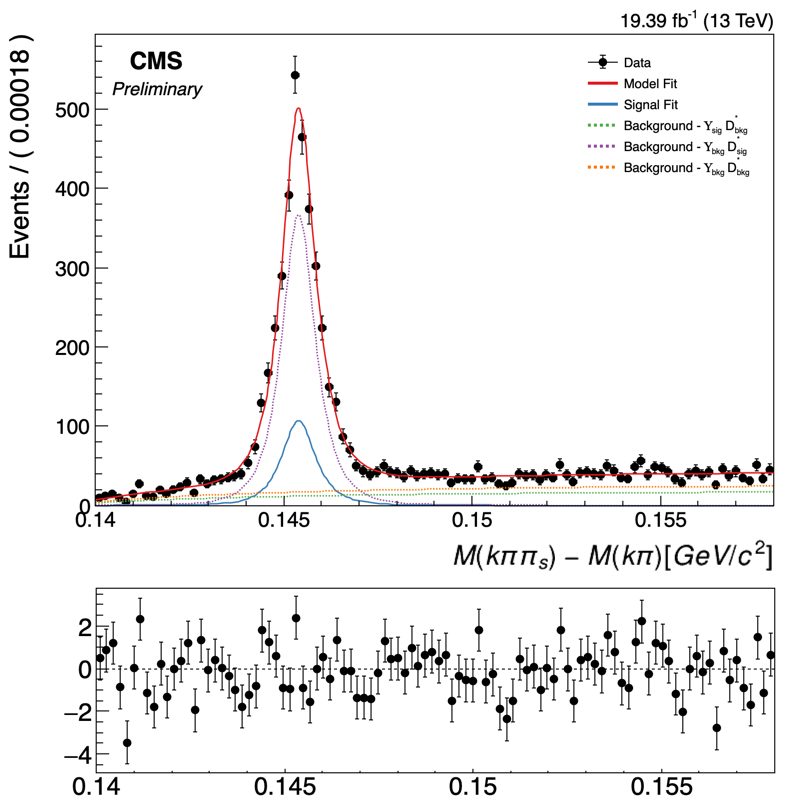
\includegraphics[width=0.23\textwidth]{figures/fit/fit2D_dstar_proj_2016APV.png}}}\hfill
    \subfloat[][2016 D$^{*\pm}$ projection.]{\label{subfig:fit2D_dstar_proj_2016}%
      \fbox{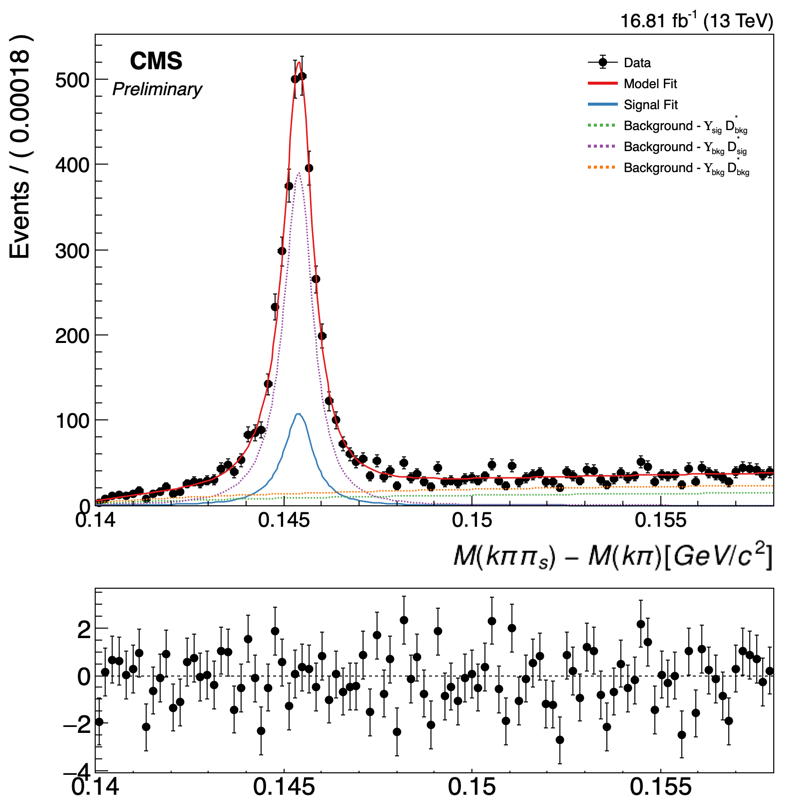
\includegraphics[width=0.23\textwidth]{figures/fit/fit2D_dstar_proj_2016.png}}}\hfill
    \subfloat[][2017 D$^{*\pm}$ projection.]{\label{subfig:fit2D_dstar_proj_2017}%
      \fbox{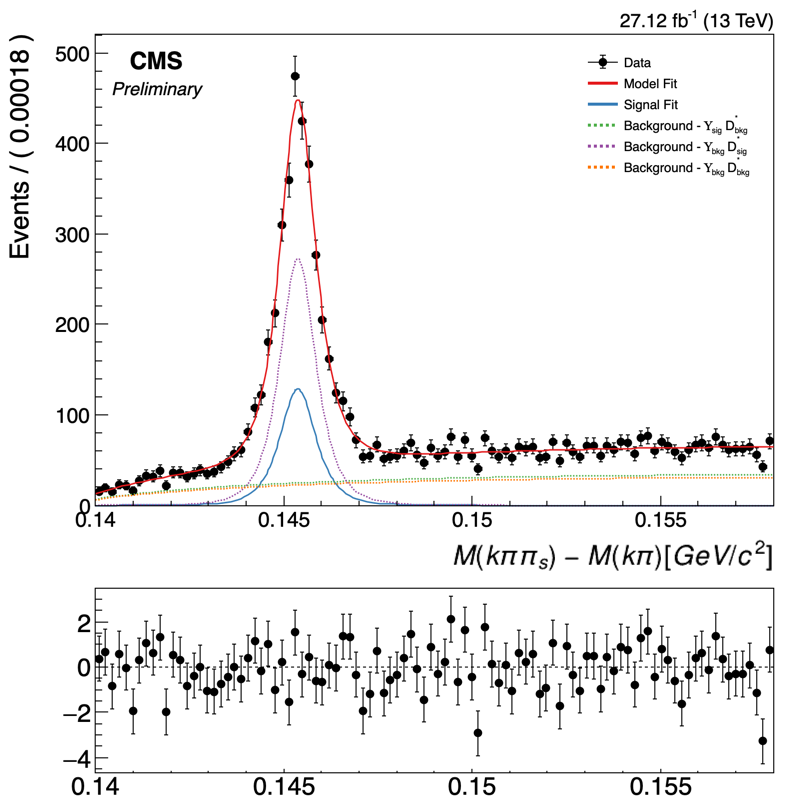
\includegraphics[width=0.23\textwidth]{figures/fit/fit2D_dstar_proj_2017.png}}}\hfill
    \subfloat[][2018 D$^{*\pm}$ projection.]{\label{subfig:fit2D_dstar_proj_2018}%
      \fbox{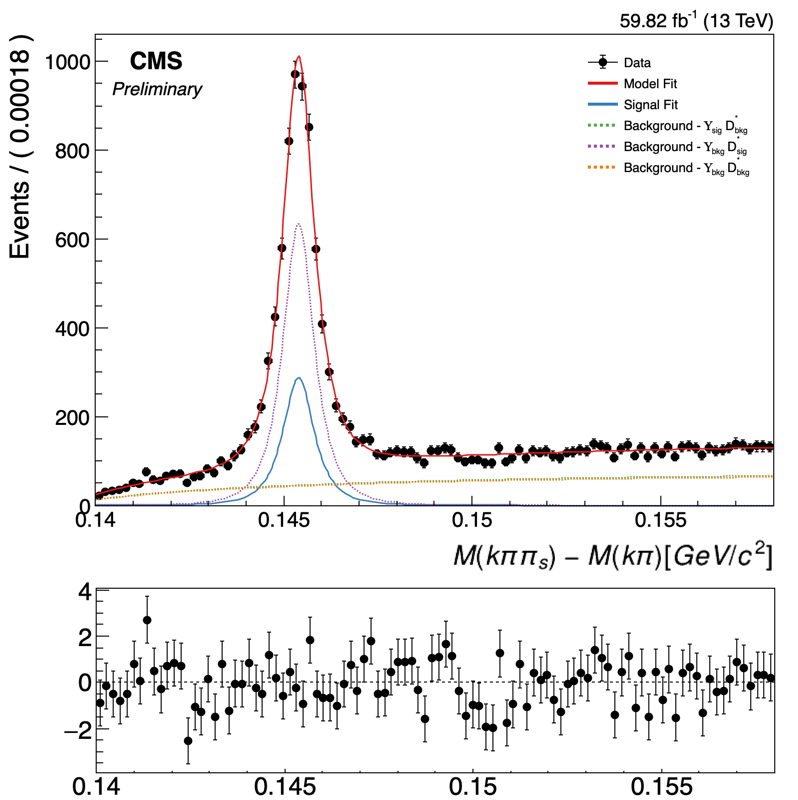
\includegraphics[width=0.23\textwidth]{figures/fit/fit2D_dstar_proj_2018.png}}}\\
    \legend{Projections to the dimuon invariant mass (a-d) and D$^{*\pm}$ $\Delta$m (e-f) taken from the fit to the selected associated $\Upsilon + $ D$^{*\pm}$ for all data samples. The curves represent the full fit (in red) and each of the components - signal in blue and continuous line and background components using dashed lines in green, purple and orange.}
  \end{figure}
\end{landscape}

The summary of the fits parameters for each of the samples are found in Tabs. \ref{tab:fit_summary_2016APV} to \ref{tab:fit_summary_2018}

\begin{table}[!htbp]{15cm}
  \caption{Summary of fit parameters for the sample 2016APV}\label{tab:fit_summary_2016APV}
  \begin{tabular}{ c | c }
    Parameter & Value \\ 
    \hline
    N$_{evt}$                    & 6785 \\ \hline
    N$_{sig} \Upsilon(1S)$       & $427 \pm 51$ \\ \hline
    N$_{sig} \Upsilon(2S)$       & $165 \pm 23$ \\ \hline
    N$_{sig} \Upsilon(3S)$       & $111 \pm 17$ \\ \hline
    m$_{scale}$                  & $0.9981 \pm 0.0004$ \\ \hline
    $\Delta$m mean               & $145.35 \pm 0.04$ MeV \\ \hline
    $\chi^2 \Upsilon$ projection & 1.55 \\ \hline
    $\chi^2 D^{*\pm}$ projection & 1.64 \\ \hline
  \end{tabular}
  \legend{A summary with the more important fit parameters for sample 2016APV.}
\end{table}

\begin{table}[!htbp]{15cm}
  \caption{Summary of fit parameters for the sample 2016}\label{tab:fit_summary_2016}
  \begin{tabular}{ c | c }
    Parameter & Value \\ 
    \hline
    N$_{evt}$                    & 6421 \\ \hline
    N$_{sig} \Upsilon(1S)$       & $479 \pm 35$ \\ \hline
    N$_{sig} \Upsilon(2S)$       & $174 \pm 17$ \\ \hline
    N$_{sig} \Upsilon(3S)$       & $141 \pm 15$ \\ \hline
    m$_{scale}$                  & $0.9981 \pm 0.0004$ \\ \hline
    $\Delta$m mean               & $145.42 \pm 0.01$ MeV \\ \hline
    $\chi^2 \Upsilon$ projection & 1.19 \\ \hline
    $\chi^2 D^{*\pm}$ projection & 1.56 \\ \hline
  \end{tabular}
  \legend{A summary with the more important fit parameters for sample 2016.}
\end{table}

\begin{table}[!htbp]{15cm}
  \caption{Summary of fit parameters for the sample 2017}\label{tab:fit_summary_2017}
  \begin{tabular}{ c | c }
    Parameter & Value \\ 
    \hline
    N$_{evt}$                    & 8454 \\ \hline
    N$_{sig} \Upsilon(1S)$       & $613 \pm 53$ \\ \hline
    N$_{sig} \Upsilon(2S)$       & $230 \pm 22$ \\ \hline
    N$_{sig} \Upsilon(3S)$       & $184 \pm 18$ \\ \hline
    m$_{scale}$                  & $0.9982 \pm 0.0003$ \\ \hline
    $\Delta$m mean               & $145.37 \pm 0.04$ MeV \\ \hline
    $\chi^2 \Upsilon$ projection & 1.07 \\ \hline
    $\chi^2 D^{*\pm}$ projection & 1.15 \\ \hline
  \end{tabular}
  \legend{A summary with the more important fit parameters for sample 2017.}
\end{table}

\begin{table}[!htbp]{15cm}
  \caption{Summary of fit parameters for the sample 2018}\label{tab:fit_summary_2018}
  \begin{tabular}{ c | c }
    Parameter & Value \\ 
    \hline 
    N$_{evt}$                    & 16765 \\ \hline
    N$_{sig} \Upsilon(1S)$       & $1200 \pm 70$ \\ \hline
    N$_{sig} \Upsilon(2S)$       & $478 \pm 31$ \\ \hline
    N$_{sig} \Upsilon(3S)$       & $310 \pm 22$ \\ \hline
    m$_{scale}$                  & $0.9987 \pm 0.0002$ \\ \hline
    $\Delta$m mean               & $145.39 \pm 0.02$ MeV \\ \hline
    $\chi^2 \Upsilon$ projection & 1.28 \\ \hline
    $\chi^2 D^{*\pm}$ projection & 1.12 \\ \hline
  \end{tabular}
  \legend{A summary with the more important fit parameters for sample 2018.}
\end{table}

\section{Acceptance and Efficiency}

The acceptance and efficiency of the process is determined from the signal MC. The strategy for computing the acceptance and efficiency is to factorize it into the components,
\begin{equation}
  (Acc\cdot\epsilon) = (Acc\cdot\epsilon_{precuts})^\Upsilon \cdot 
  (Acc\cdot\epsilon_{precuts})^{D^*} \cdot \epsilon_{cuts}^\Upsilon \cdot 
  \epsilon_{cuts}^{D^*} \cdot \epsilon_{HLT} \cdot \epsilon_{association},
\end{equation}
where the $Acc\cdot\epsilon_{precuts}$ is the acceptance coupled to the precuts efficiency, $\epsilon_{cuts}$ is the selection cuts efficiency, $\epsilon_{HLT}$ is the trigger efficiency and the $\epsilon_{association}$ is the efficiency related to the $\Upsilon+D^*$ association criteria. Sec. \ref{sec:evtsel} gives details of the precuts and cuts applied.

Each of the components are calculated to create two dimensional maps used to extract the efficiency of the data samples.

\subsection{Acceptance}

The acceptance is calculated taking into account the precuts (Tab. \ref{tab:preselectioncuts}) and the cuts that define the fiducial volume of the sample on Tab. \ref{tab:fiducialvol}. The acceptance coupled to the precuts is calculated by
\begin{equation}
    (Acc \cdot \epsilon_{precuts})^P = \frac{N_{reco}^P}{N_{gen}^P},
\end{equation}
where the superscript P refers either to $\Upsilon$ or D$^*$, $N_{gen}$ is the number of generated particles within the fiducial volume, and $N_{reco}$ is the number of reconstructed particles within the same fiducial volume, passing the precuts and satisfying the respective matching criteria for that kind of particle:
\begin{itemize}
  \item For $\Upsilon$: the two muons used for its reconstruction must be matched to the muons from the decay of the generated Y within a cone of $\Delta R = \sqrt{\Delta \eta^2 + \Delta \phi^2} < 0.03$.
  \item For $D^*$: The reconstructed $D^*$ matches the generated $D^*$ with the requirements:
  $$\frac{|p_T^{reco} - p_T^{gen}|}{p_T^{gen}} < 0.2, |\eta_{gen} - \eta_{reco}|
  < 0.3, remainder(|\phi_{gen} - \phi_{reco}|, 2\pi) < 0.3.$$
\end{itemize}

The plots of the acceptance extracted from the 2018 MC sample are given in Figs. \ref{fig:acc_dimu} and \ref{fig:acc_dstar} for $\Upsilon$ and D$^*$, respectively.

\begin{figure}[!htm]{15cm}
  \caption{$\Upsilon$ acceptance of the selected associated $\Upsilon +$ D$^*$ extracted from 2018 MC sample.} 
  \label{fig:acc_dimu}
  \subfloat[][]{\label{subfig:acc_dimu_pt}%
    \fbox{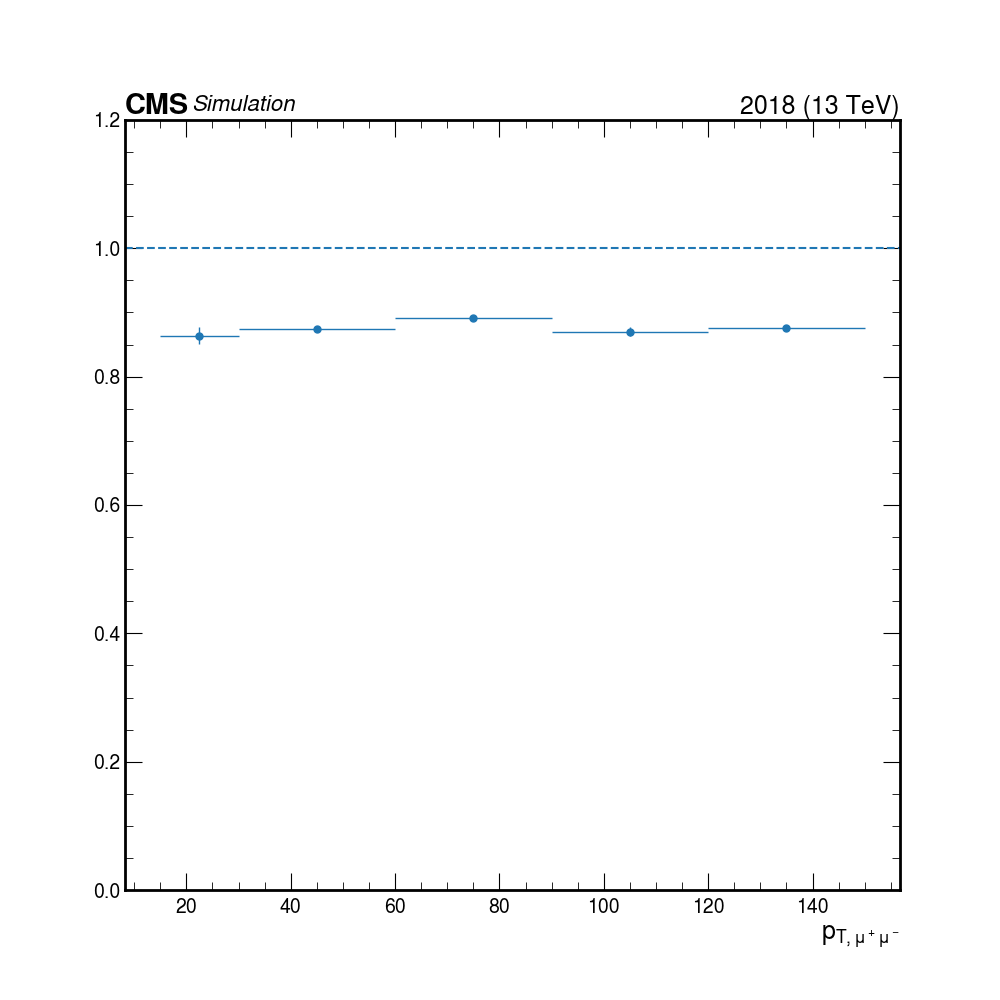
\includegraphics[width=0.47\textwidth]{figures/efficiency/acc_dimu_pt_2018.png}}}\hfill
  \subfloat[][]{\label{subfig:acc_dimu_rap}%
    \fbox{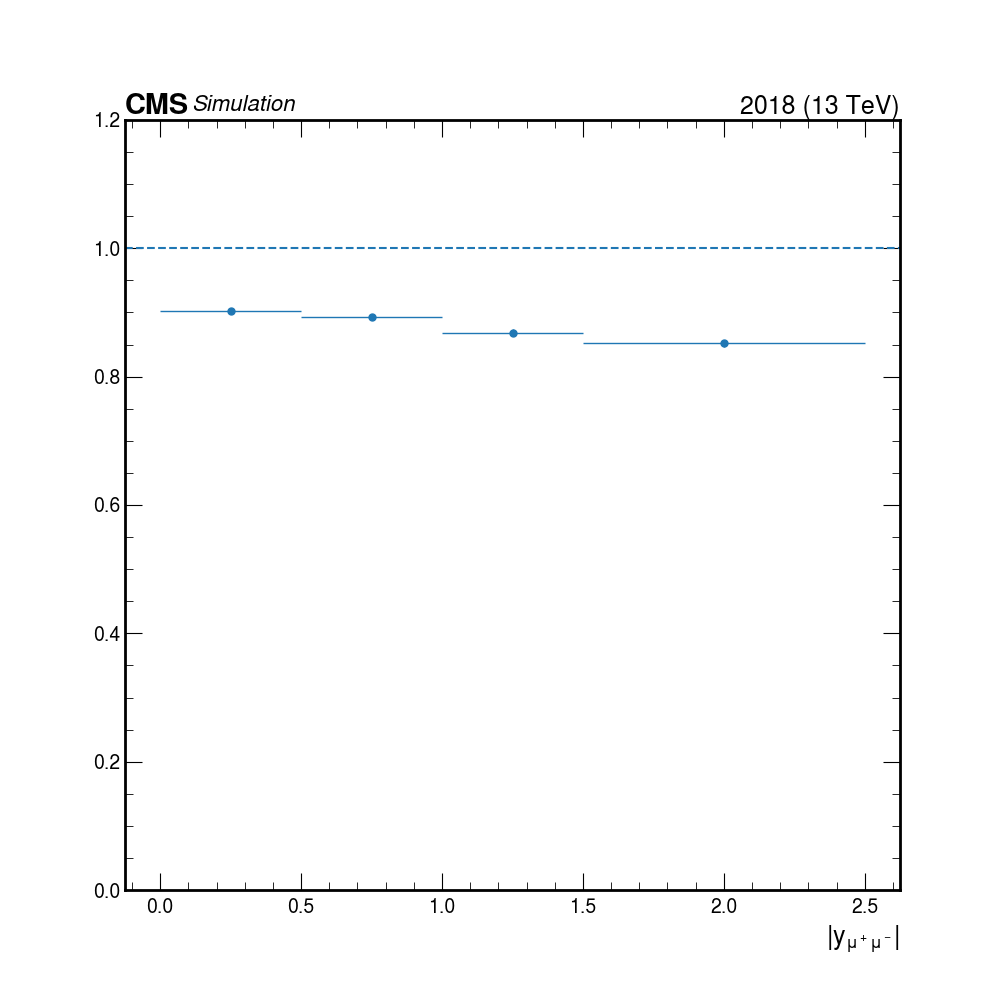
\includegraphics[width=0.47\textwidth]{figures/efficiency/acc_dimu_rap_2018.png}}}\hfill\\
    \subfloat[][]{\label{subfig:acc_dimu_2D}%
    \fbox{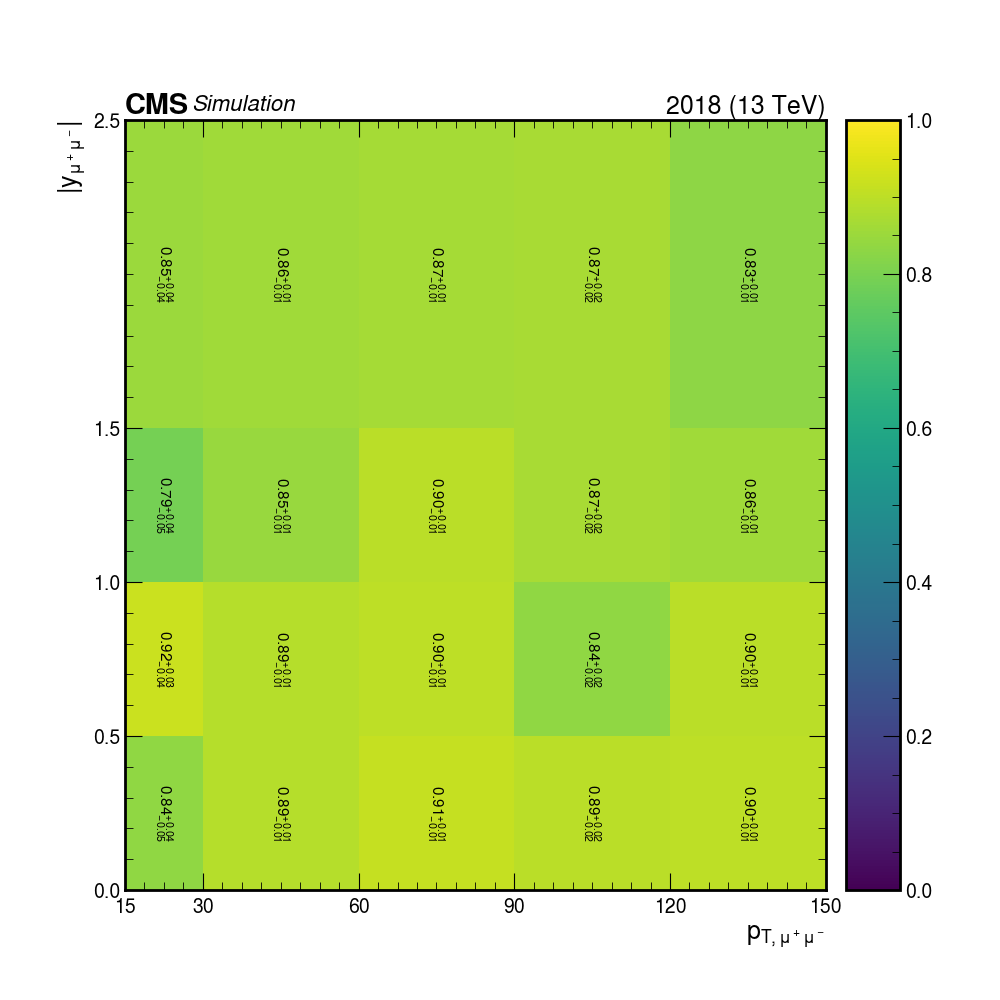
\includegraphics[width=0.47\textwidth]{figures/efficiency/acc_dimu_2018.png}}}\\
  \legend{$\Upsilon$ acceptance extracted from the 2018 MC data sample. The acceptance is given with respect to the dimuon $p_T$ in (a), $y$ in (b), and in both $p_T$ and $y$ in (c). In (a) and (b). The horizontal dashed line is set to the upper limit of the acceptance, one.}
\end{figure}

\begin{figure}[!htm]{15cm}
  \caption{D$^*$ acceptance of the selected associated $\Upsilon +$ D$^*$ extracted from 2018 MC sample.} 
  \label{fig:acc_dstar}
  \subfloat[][]{\label{subfig:acc_dstar_pt}%
    \fbox{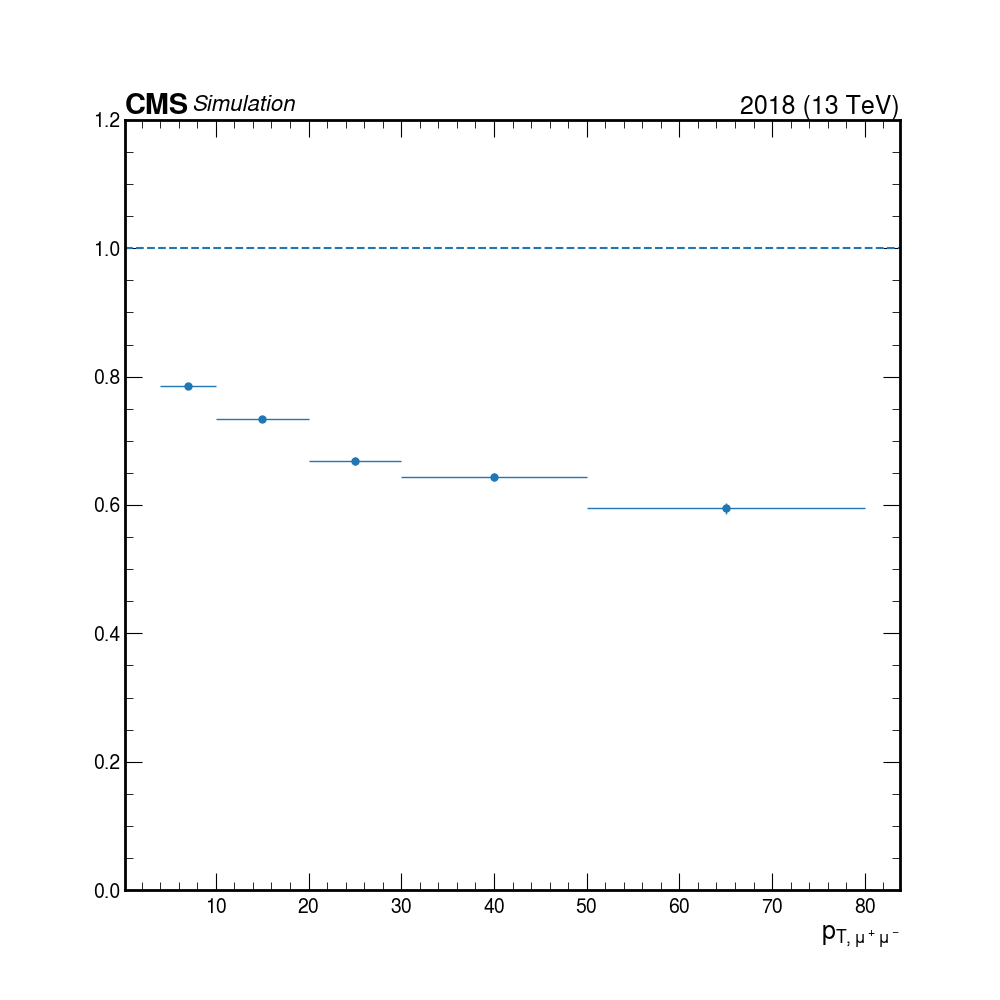
\includegraphics[width=0.47\textwidth]{figures/efficiency/acc_dstar_pt_2018.png}}}\hfill
  \subfloat[][]{\label{subfig:acc_dstar_rap}%
    \fbox{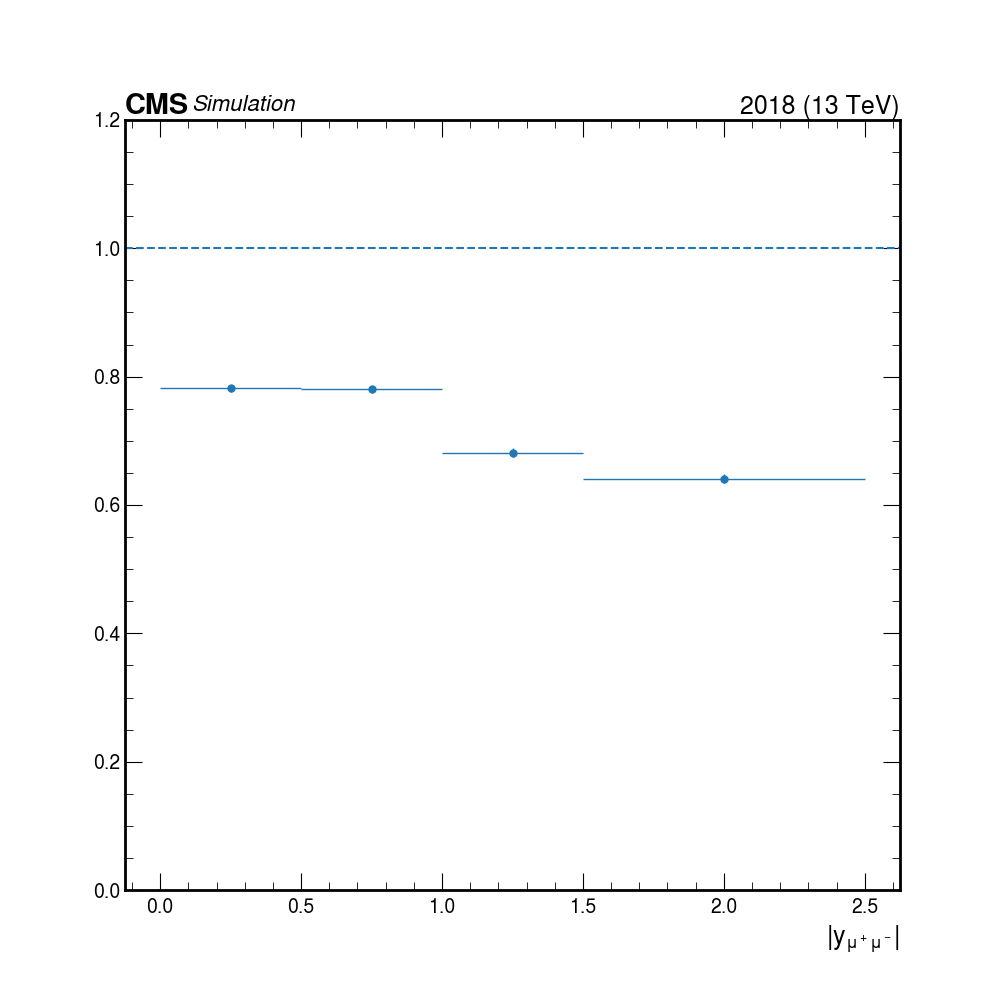
\includegraphics[width=0.47\textwidth]{figures/efficiency/acc_dstar_rap_2018.png}}}\hfill\\
    \subfloat[][]{\label{subfig:acc_dstar_2D}%
    \fbox{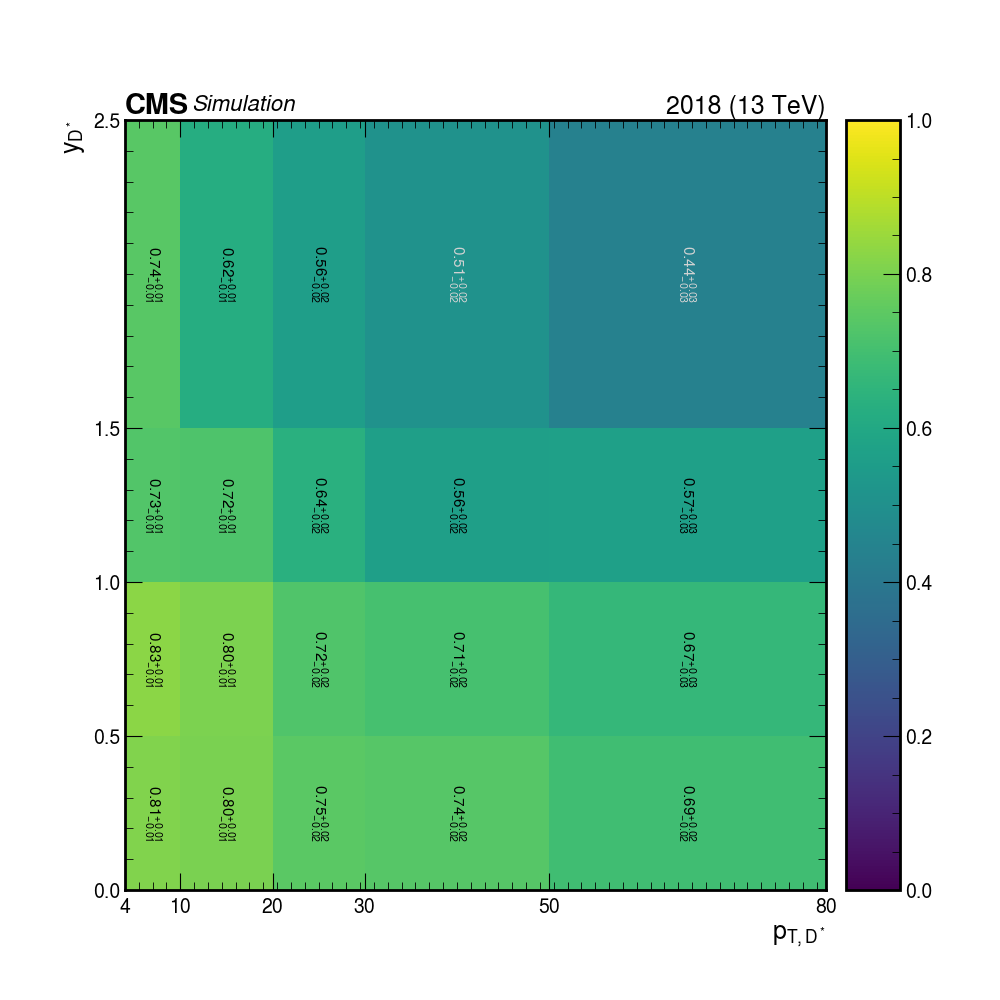
\includegraphics[width=0.47\textwidth]{figures/efficiency/acc_dstar_2018.png}}}\\
  \legend{D$^*$ acceptance extracted from the 2018 MC data sample. The acceptance is given with respect to the reconstructed D$^*$ $p_T$ in (a), $y$ in (b), and in both $p_T$ and $y$ in (c). In (a) and (b). The horizontal dashed line is set to the upper limit of the acceptance, one.}
\end{figure}

\subsection{Selection Cuts Efficiency}

The cuts considered for this efficiency component are the ones stated in the Tab. \ref{tab:selectioncuts} with exception to the cut on the $\mu\mu\pi_s$ vertex probability cut, which is treated separately. The denominator is the number of reconstructed events that passed the precuts criteria and the numerator is the number of events that passed the cuts and the precuts:
\begin{equation}
  \epsilon_{cuts}^P = \frac{N_{reco\&cuts}^P}{N_{reco}^P} (P = \Upsilon, D^*).
\end{equation}

The plots of the selection cuts efficiency extracted from the 2018 MC sample are given in Figs. \ref{fig:eff_cuts_dimu} and \ref{fig:eff_cuts_dstar} for $\Upsilon$ and D$^*$, respectively.

\begin{figure}[!htm]{15cm}
  \caption{$\Upsilon$ selection cuts efficiency of the selected associated $\Upsilon +$ D$^*$ extracted from 2018 MC sample.} 
  \label{fig:eff_cuts_dimu}
  \subfloat[][]{\label{subfig:eff_cuts_dimu_pt}%
    \fbox{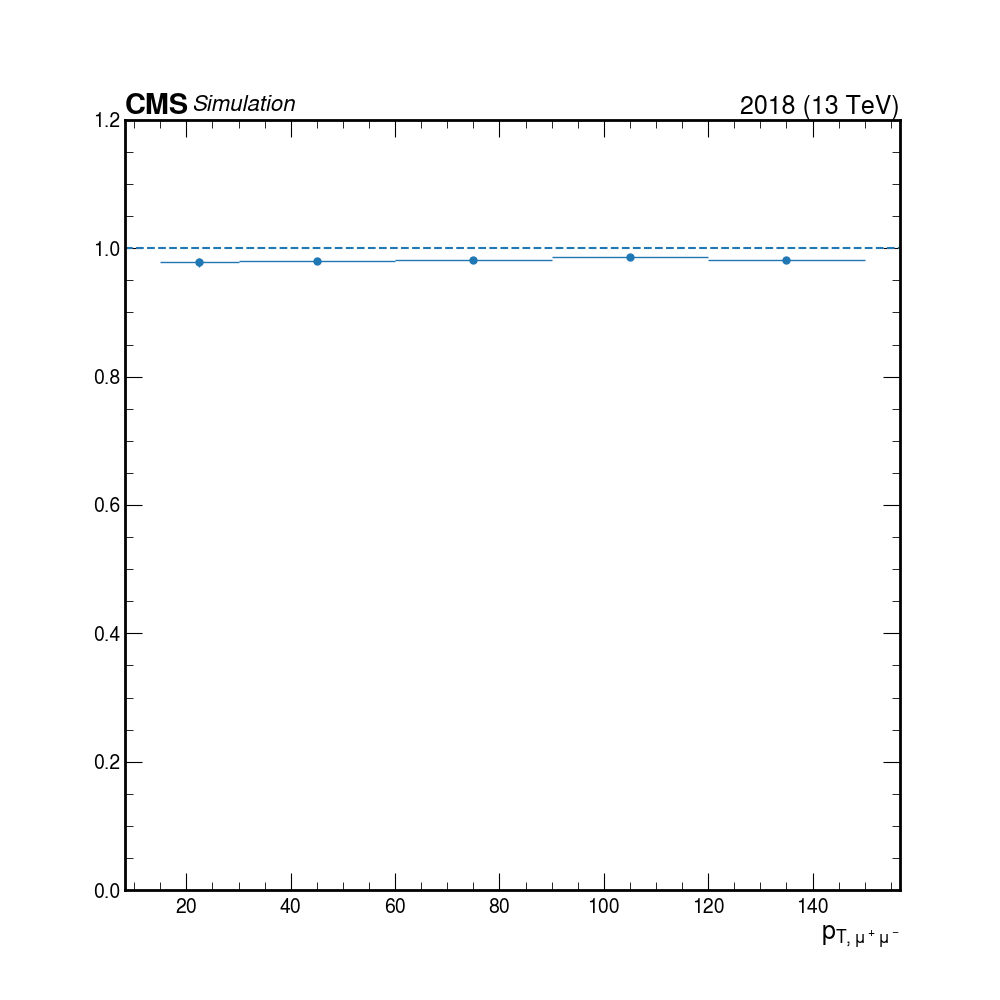
\includegraphics[width=0.47\textwidth]{figures/efficiency/eff_cuts_dimu_pt_2018.png}}}\hfill
  \subfloat[][]{\label{subfig:eff_cuts_dimu_rap}%
    \fbox{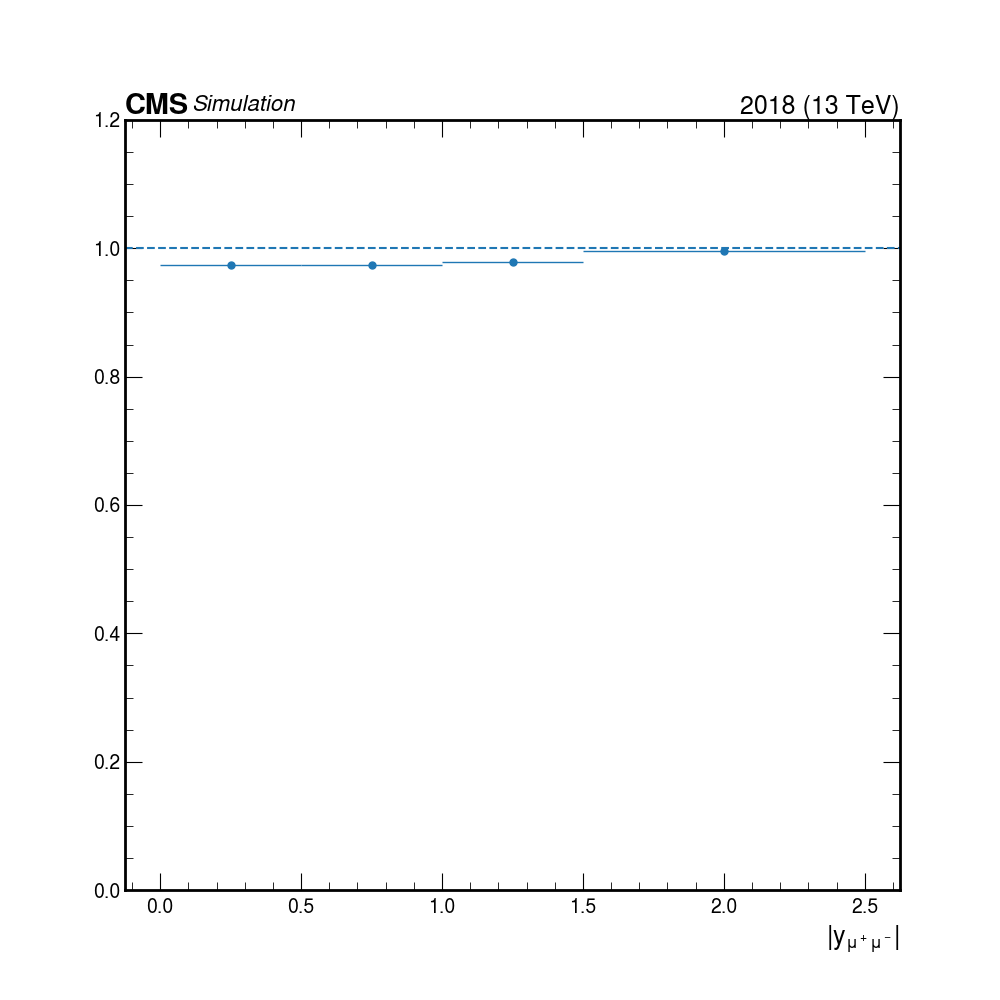
\includegraphics[width=0.47\textwidth]{figures/efficiency/eff_cuts_dimu_rap_2018.png}}}\hfill\\
    \subfloat[][]{\label{subfig:eff_cuts_dimu_2D}%
    \fbox{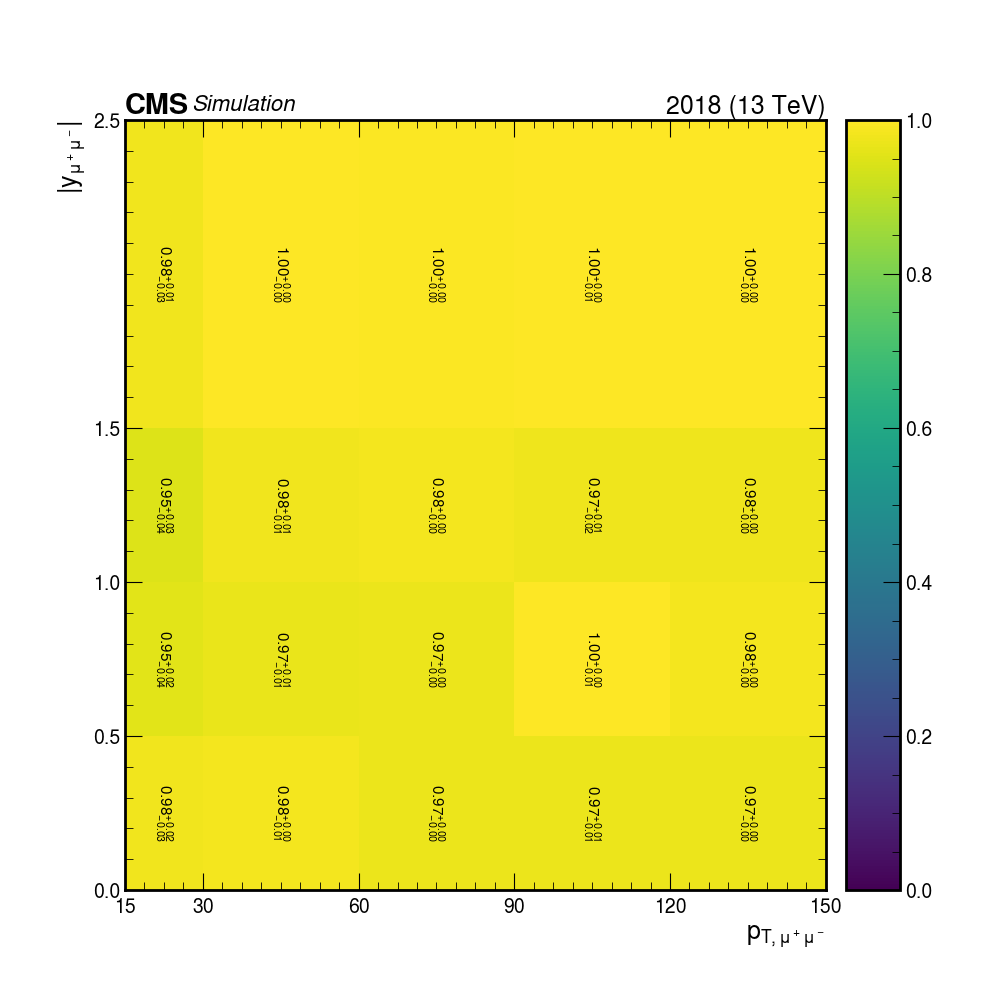
\includegraphics[width=0.47\textwidth]{figures/efficiency/eff_cuts_dimu_2018.png}}}\\
  \legend{$\Upsilon$ selection cuts efficiency extracted from the 2018 MC data sample. This efficiency is given with respect to the dimuon $p_T$ in (a), $y$ in (b), and in both $p_T$ and $y$ in (c). In (a) and (b). The horizontal dashed line is set to the upper limit of the efficiency.}
\end{figure}

\begin{figure}[!htm]{15cm}
  \caption{D$^*$ selection cuts efficiency of the selected associated $\Upsilon +$ D$^*$ extracted from 2018 MC sample.} 
  \label{fig:eff_cuts_dstar}
  \subfloat[][]{\label{subfig:eff_cuts_dstar_pt}%
    \fbox{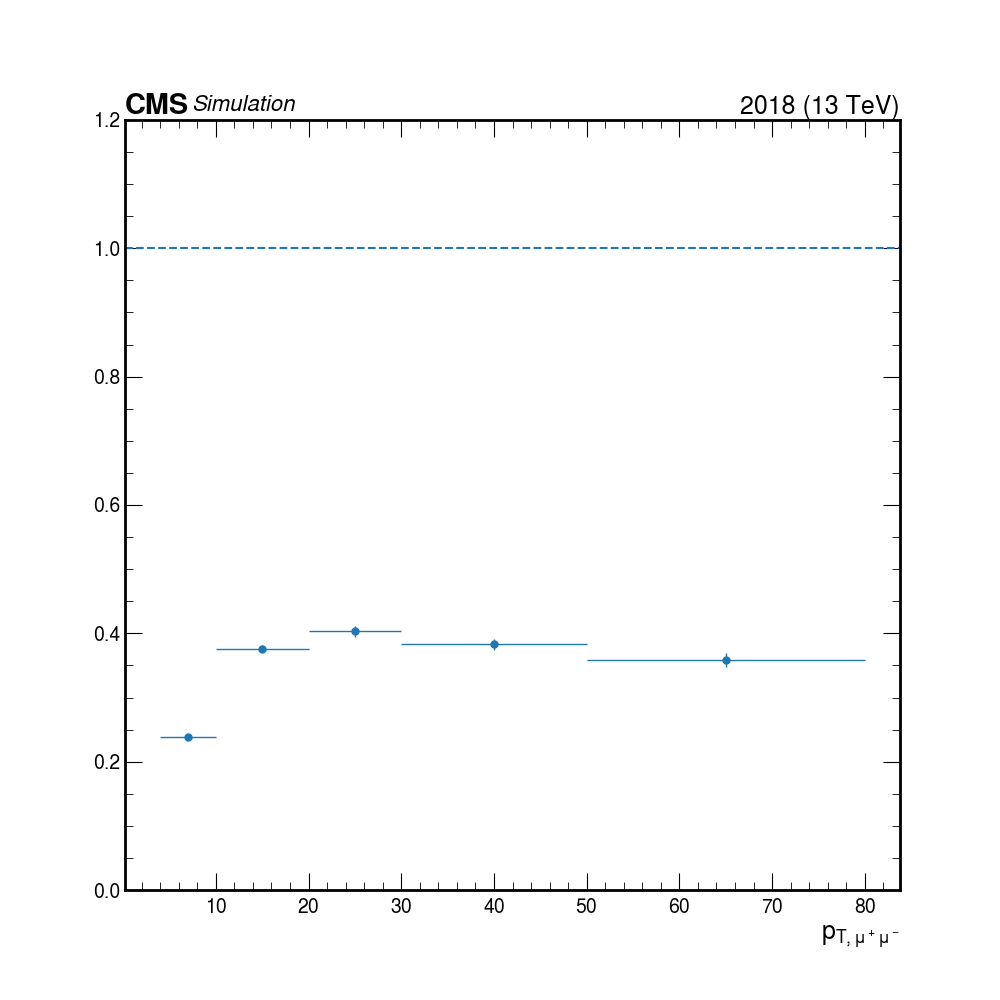
\includegraphics[width=0.47\textwidth]{figures/efficiency/eff_cuts_dstar_pt_2018.png}}}\hfill
  \subfloat[][]{\label{subfig:eff_cuts_dstar_rap}%
    \fbox{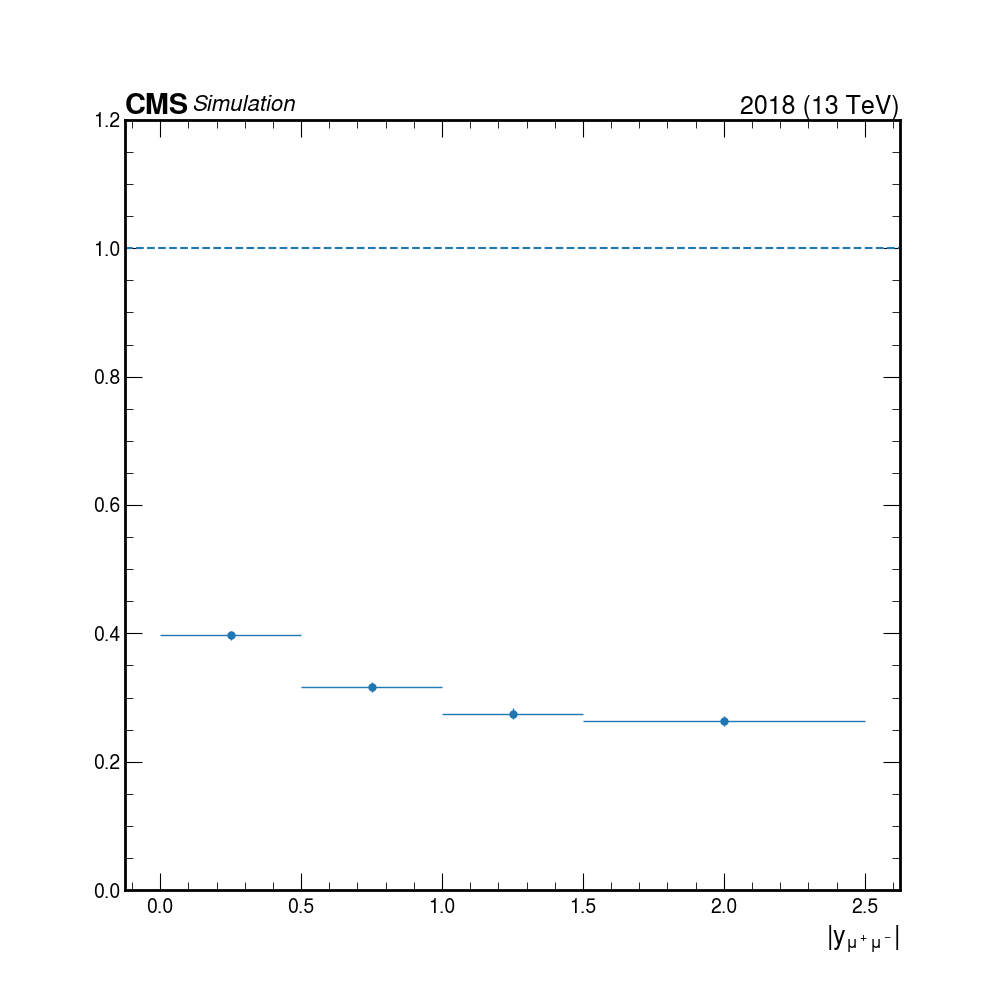
\includegraphics[width=0.47\textwidth]{figures/efficiency/eff_cuts_dstar_rap_2018.png}}}\hfill\\
    \subfloat[][]{\label{subfig:eff_cuts_dstar_2D}%
    \fbox{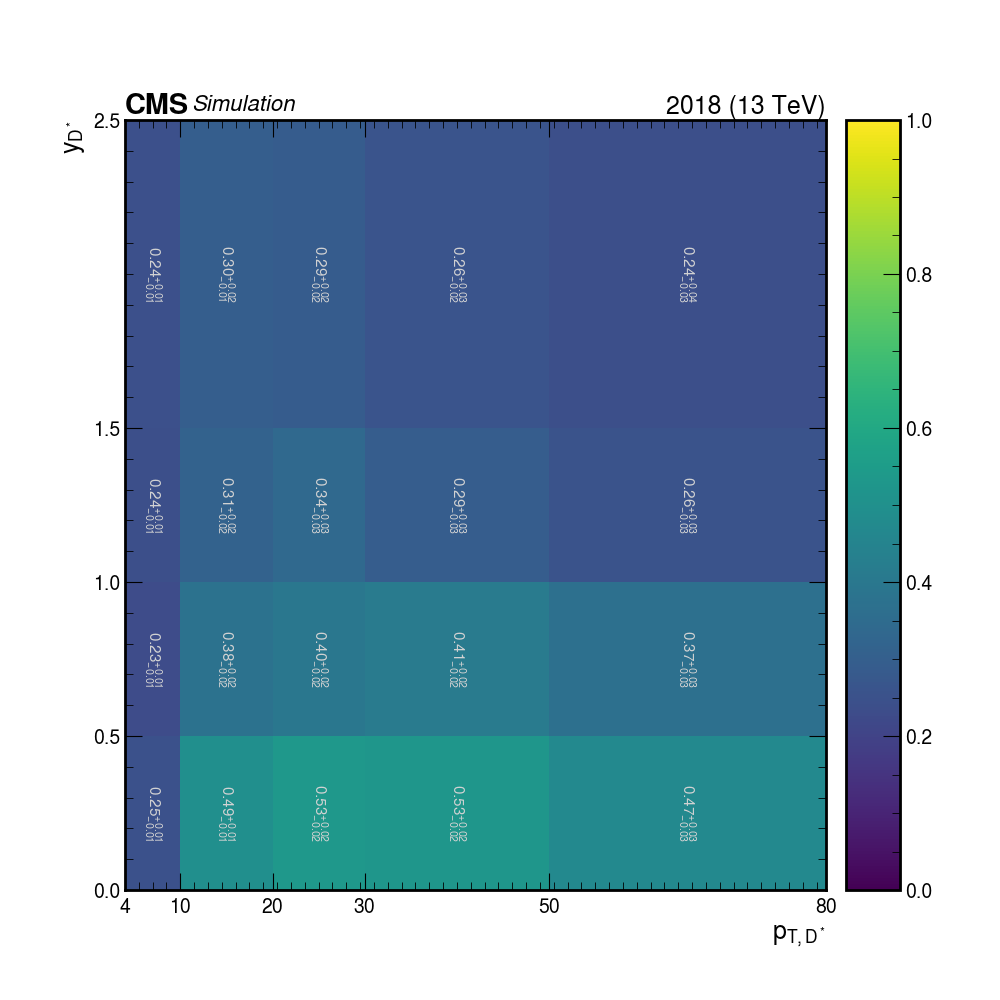
\includegraphics[width=0.47\textwidth]{figures/efficiency/eff_cuts_dstar_2018.png}}}\\
  \legend{D$^*$ selection cuts efficiency extracted from the 2018 MC data sample. This efficiency is given with respect to the D$^*$ $p_T$ in (a), $y$ in (b), and in both $p_T$ and $y$ in (c). In (a) and (b). The horizontal dashed line is set to the upper limit of the efficiency.}
\end{figure}

\subsection{Trigger Efficiency}

The triggers used depend only on the dimuons, therefore, their efficiency is only evaluated from the $\Upsilon$ candidates. The denominator is the number of events that passed both the precuts and cuts criteria and the numerator the number of events passing the trigger, cuts and precuts:
\begin{equation}
  \epsilon_{HLT} = \frac{N_{reco\&cuts\&trigger}^\Upsilon}{N_{reco\&cuts}^\Upsilon}
\end{equation}

The plots of the trigger efficiency extracted from the 2018 MC sample are given in Fig. \ref{fig:eff_trigger}.

\begin{figure}[!htm]{15cm}
  \caption{Trigger efficiency of the selected associated $\Upsilon +$ D$^*$ extracted from 2018 MC sample.} 
  \label{fig:eff_trigger}
  \subfloat[][]{\label{subfig:eff_trigger_pt}%
    \fbox{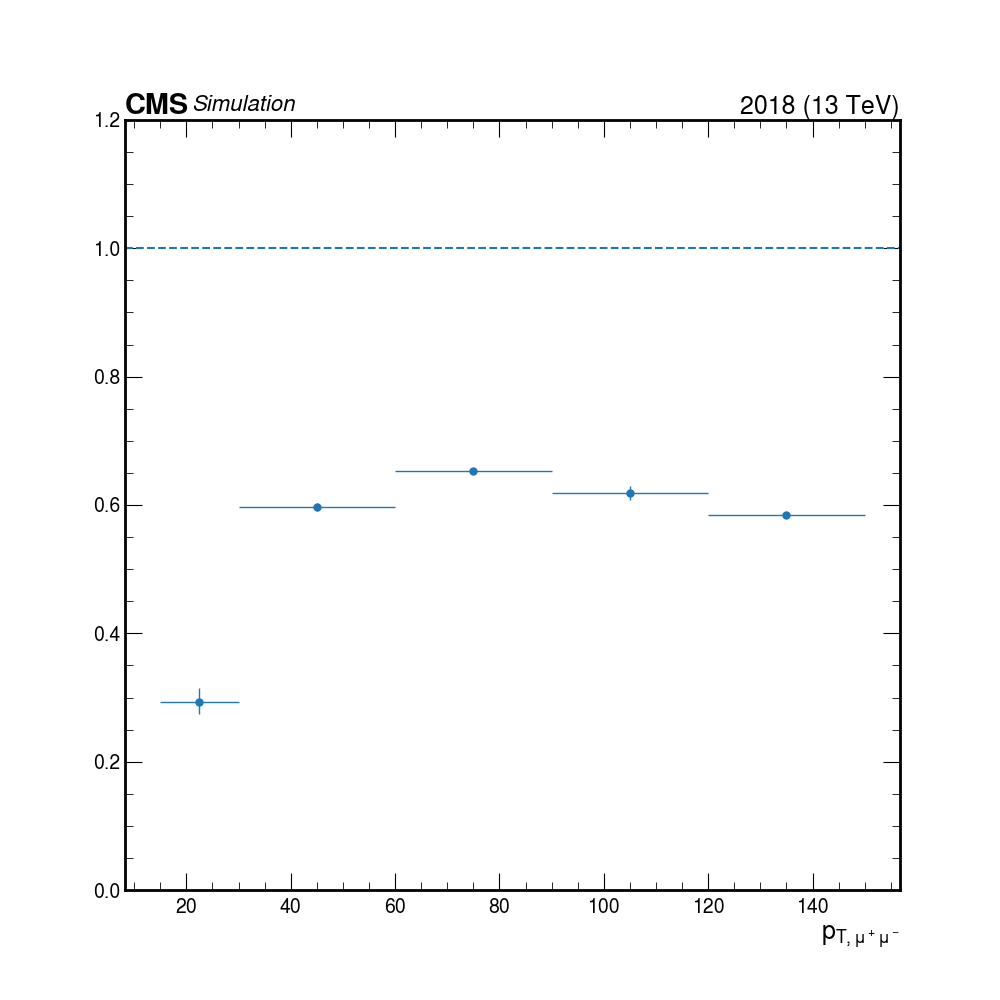
\includegraphics[width=0.47\textwidth]{figures/efficiency/eff_trigger_pt_2018.png}}}\hfill
  \subfloat[][]{\label{subfig:eff_trigger_rap}%
    \fbox{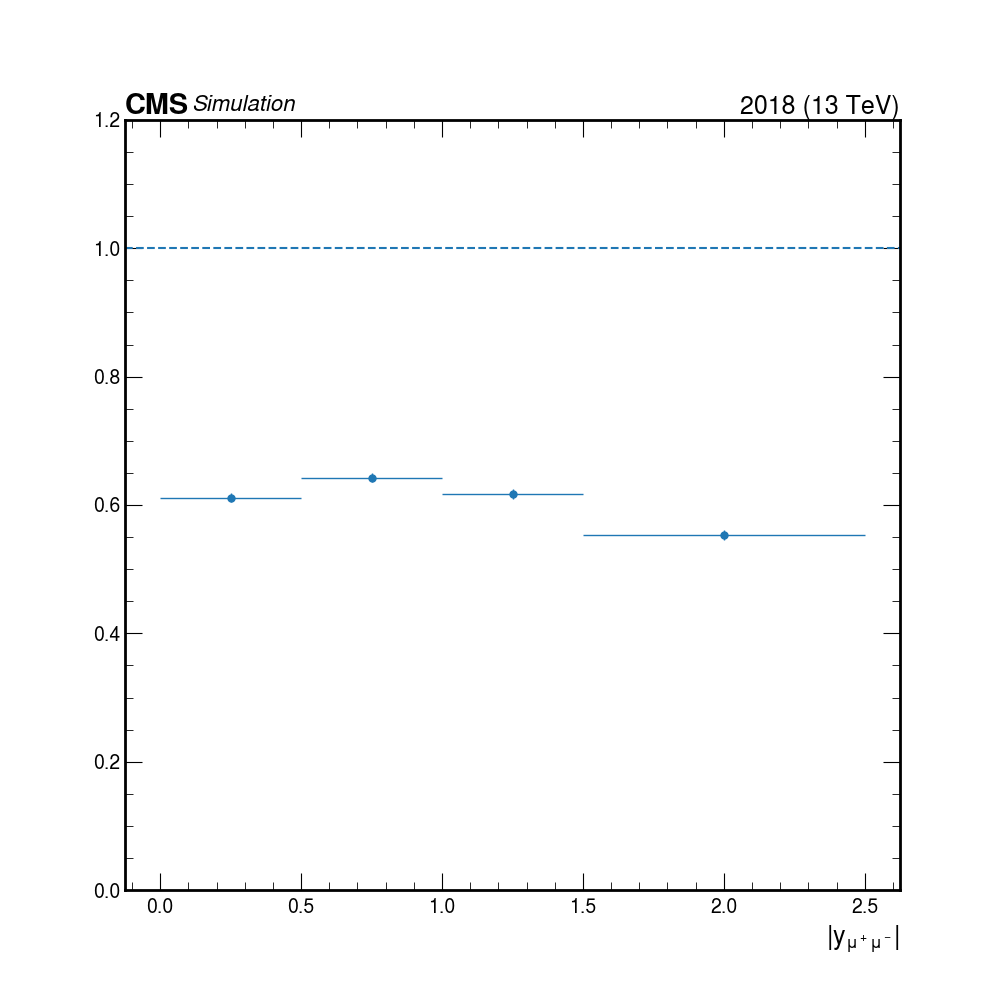
\includegraphics[width=0.47\textwidth]{figures/efficiency/eff_trigger_rap_2018.png}}}\hfill\\
    \subfloat[][]{\label{subfig:eff_trigger_2D}%
    \fbox{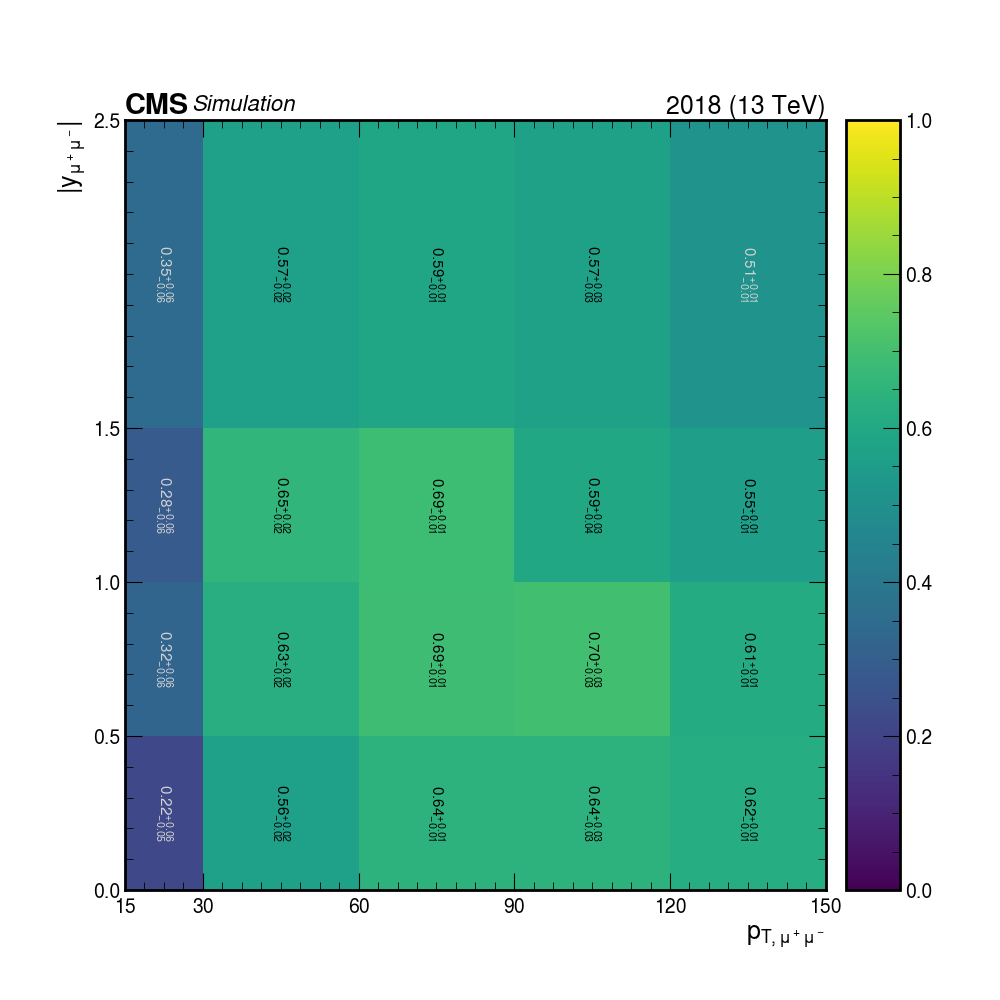
\includegraphics[width=0.47\textwidth]{figures/efficiency/eff_trigger_2018.png}}}\\
  \legend{Trigger efficiency extracted from the 2018 MC data sample. This efficiency is given with respect to the dimuon $p_T$ in (a), $y$ in (b), and in both $p_T$ and $y$ in (c). In (a) and (b). The horizontal dashed line is set to the upper limit of the efficiency.}
\end{figure}

\subsection{Association efficiency}

The last efficiency is related to the association between $\Upsilon$ and $D^*$. It is given by
\begin{equation}
  \epsilon_{association} = 
  \frac{N_{reco\&cuts\&trigger\&association}^{\Upsilon D^*}}{N_{reco\&cuts\&trigger}^{\Upsilon D^*}},
\end{equation}
where the denominator is the number events that passed all the previous selections and the numerator is the number of events after the addition of the association cut, which is the $\mu\mu\pi_s$ vertex probability $> 0.01$.

The plots of the trigger efficiency extracted from the 2018 MC sample are given in Fig. \ref{fig:eff_asso}.

\begin{figure}[!htm]{15cm}
  \caption{Trigger efficiency of the selected associated $\Upsilon +$ D$^*$ extracted from 2018 MC sample.} 
  \label{fig:eff_asso}
  \subfloat[][]{\label{subfig:eff_asso_pt}%
    \fbox{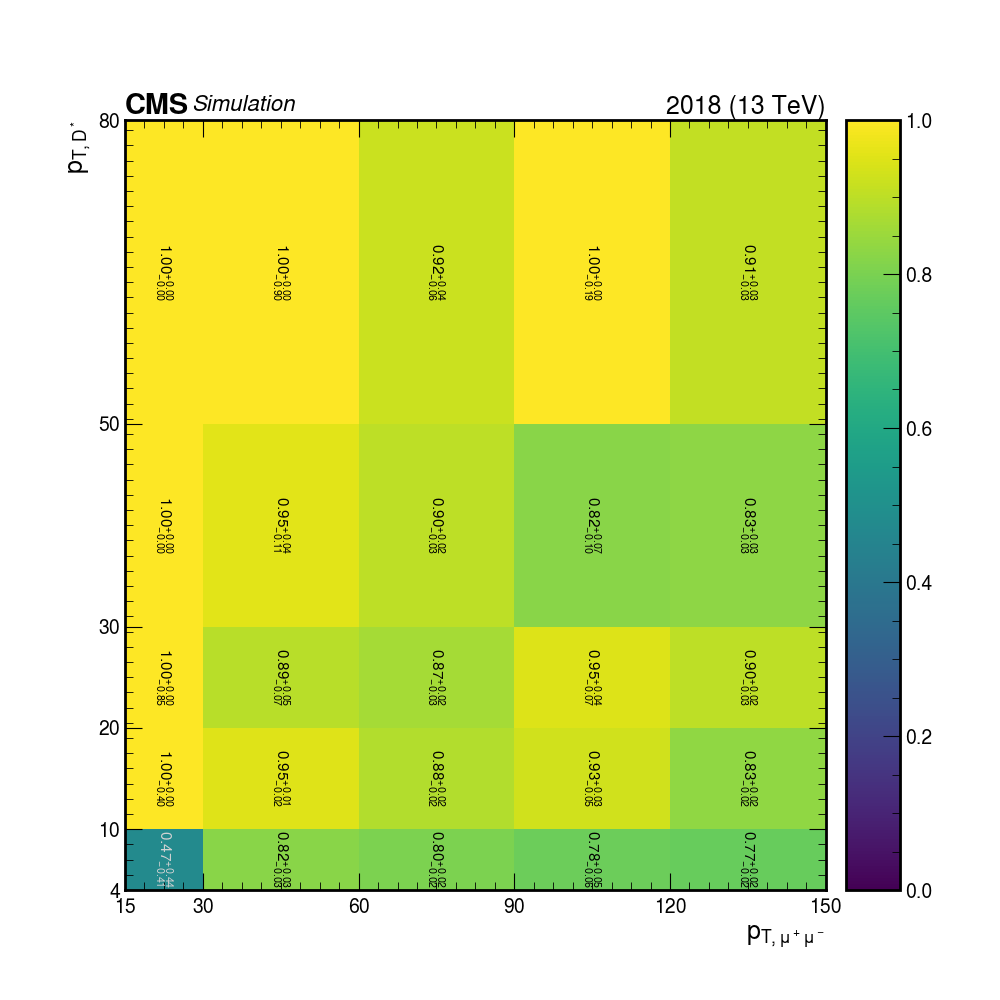
\includegraphics[width=0.47\textwidth]{figures/efficiency/eff_asso_pt_2018.png}}}\hfill
  \subfloat[][]{\label{subfig:eff_asso_rap}%
    \fbox{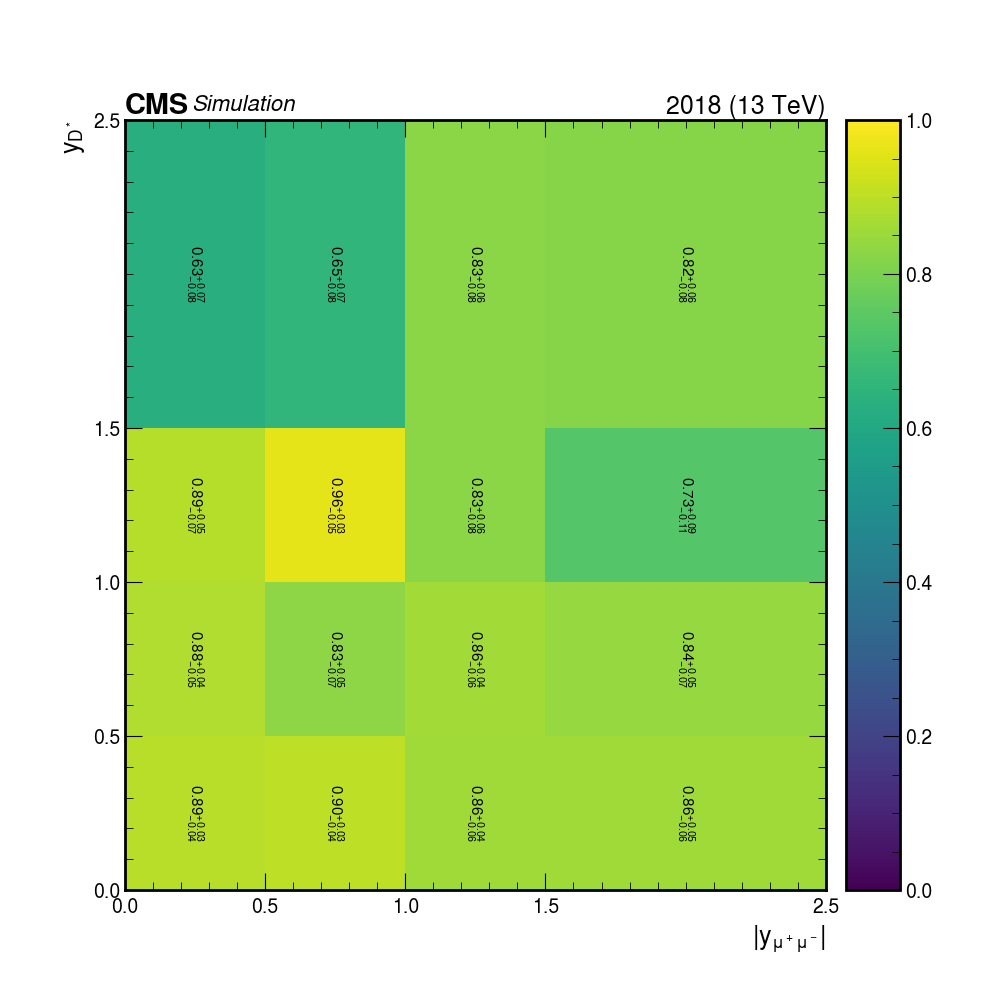
\includegraphics[width=0.47\textwidth]{figures/efficiency/eff_asso_rap_2018.png}}}\hfill\\
  \legend{Associuation efficiency extracted from the 2018 MC data sample. The efficiency maps are given with respect to the dimuon and D$^*$ $p_T$ in (a) and $y$ in (b).}
\end{figure}

\subsection{Total efficiency}\label{sec:total_eff}

The shown efficiency maps are used to calculate efficiency that will be used in the cross section determination. The final efficiency for each subsample is shown in Tab. \ref{tab:totaleff}.

\begin{table}[!htbp]{15cm}
  \caption{Total efficiency per data sample.}
  \begin{tabular}{ l | c }
    \hline
    \multicolumn{1}{c|}{Sample} & \multicolumn{1}{c}{Total Efficiency (\%)} \\ \hline
    2016APV & $7.5^{+1.0}_{-1.6}$ \\ \hline
    2016    & $9.3^{+1.1}_{-2.6}$ \\ \hline
    2017    & $6.9^{+1.2}_{-1.7}$ \\ \hline
    2018    & $4.4^{+1.5}_{-1.7}$ \\ \hline
  \end{tabular}
  \legend{Total efficiency per data sample. The uncertainties shown are only statistical.}
  \label{tab:totaleff}
\end{table}

It is worth noting that the efficiencies displayed here are measured using a private MC with reduced statistics, resulting in a bigger uncertainties, in special for the sample 2018, with uncertainty of $\approx$ 30 \%. A new generation, with higher statistics is being processed, so it is expected that the efficiency will be better determined in the future.

\section{Associated \texorpdfstring{$\Upsilon(nS)$ + D$^{*}$}{Y+D*} Cross Section}

\subsection{Fiducial Cross Section} \label{subsec:fiducial_xsec}

The cross section of the associated $\Upsilon$ + D$^{*}$ is calculated by the formula:
\begin{equation}
  \sigma_{\Upsilon(nS) D^*} = \frac{N_{\Upsilon(nS) D^*}}{L\cdot eff \cdot BR(\Upsilon(nS))BR(D^*)},
\end{equation}
where $nS$ refers to the $\Upsilon$ states (1S, 2S and 3S), $N_{\Upsilon(nS) D^*}$ is the number of associated $\Upsilon(nS)$ + D$^*$ extracted from the 2D fit, $L$ is the integrated luminosity of the sample (Sec. \ref{sec:trigger}), $eff$ is the total efficiency (Sec. \ref{sec:total_eff}) and $BR(\Upsilon(nS))$ and $BR(D^*)$ are the branch ratios of $\Upsilon$ and D$^*$, respectively.

Table \ref{tab:DPS_xsec} presents the fiducial cross section for each data sample and $\Upsilon$ state. The values are compatible with each other so that the can be combined.

\begin{table}[!htbp]{15cm}
  \caption{$\Upsilon(nS)$ + D$^{*}$ fiducial cross section per data sample.}
  \begin{tabular}{ l | l | c }
    \hline
    Associated measurement & Sample & Cross section (pb) \\ \hline
    \multirow[c]{4}{*}{$\Upsilon(1S)$ + D$^{*\pm}$} 
    & 2016APV & $444^{+77}_{-107}$ \bigstrut\\\cline{2-3} 
    & 2016    & $462^{+66}_{-134}$ \bigstrut\\\cline{2-3} 
    & 2017    & $495^{+96}_{-128}$ \bigstrut\\\cline{2-3} 
    & 2018    & $680^{+237}_{-266}$ \\ \hline
    \multirow[c]{4}{*}{$\Upsilon(2S)$ + D$^{*\pm}$} 
    & 2016APV & $221^{+41}_{-55}$ \bigstrut\\\cline{2-3} 
    & 2016    & $216^{+34}_{-64}$ \bigstrut\\\cline{2-3} 
    & 2017    & $239^{+47}_{-62}$ \bigstrut\\\cline{2-3} 
    & 2018    & $349^{+122}_{-137}$ \\ \hline
    \multirow[c]{4}{*}{$\Upsilon(3S)$ + D$^{*\pm}$} 
    & 2016APV & $131^{+26}_{-34}$ \bigstrut\\\cline{2-3} 
    & 2016    & $155^{+25}_{-47}$ \bigstrut\\\cline{2-3} 
    & 2017    & $169^{+34}_{-44}$ \bigstrut\\\cline{2-3} 
    & 2018    & $200^{+70}_{-79}$ \\ \hline
  \end{tabular}
  \legend{$\Upsilon(nS)$ + D$^{*}$ cross section per data sample. The cross section is determined for each of the $\Upsilon$ states and its uncertainties are only statistical.}
  \label{tab:DPS_xsec}
\end{table}

Finally, the combined cross section for each $\Upsilon$ state are:
\begin{equation}
\begin{split}
  \sigma_{Y(1S)D^{*\pm}} &= 474^{+44}_{-68} \; \text{pb},\\
  \sigma_{Y(2S)D^{*\pm}} &= 230^{+23}_{-34} \; \text{pb},\\
  \sigma_{Y(3S)D^{*\pm}} &= 152^{+16}_{-22} \; \text{pb},
\end{split} 
\end{equation}
where only statistical errors are considered.

\subsection{Effective Cross Section}

The effective cross section can be determined by rearranging the Eq. \ref{eq:xsecDPS}
\begin{equation}
  \sigma_{eff} = \frac{\sigma_\Upsilon \cdot \sigma_{D^*}}{\sigma_{\Upsilon D^*}^{DPS}}.
\end{equation}
The $\sigma^{DPS}$ is different from the cross section determined in Sec. \ref{subsec:fiducial_xsec}, as this one is composed from the SPS and DPS components. It is possible to write
\begin{equation}
  \sigma_{\Upsilon D^*} = \sigma_{\Upsilon D^*}^{SPS} + \sigma_{\Upsilon D^*}^{DPS}.
\end{equation}
To calculate the $\sigma_{eff}$, the fraction of the DPS contribution needs to be computed, which is normally done by inspection of the $\Delta$y and/or $\Delta\phi$ distributions \cite{Lansberg:2019adr}. In this work, the fraction is assumed to be one, and the value presented can be assumed as a lower bound for the $\sigma_{eff}$.

The inclusive cross section of $\Upsilon(nS)$ and D$^*$ can be found in Tab. \ref{tab:inclusive_xsec}.

\begin{table}[!htbp]{15cm}
  \caption{Fiducial cross section of $\Upsilon(nS)$ and D$^*$.}
  \begin{tabular}{ c | c | c }
    \hline
    Particle & Fiducial cross section & Kinematic region \\ \hline
    $\Upsilon(1S)$ & $87.7 \pm 1.4 \text{(stat)} \pm 5.3 \text{(syst)}$ pb  & \multirow[c]{3}{*}{$20 < p_T < 130$ GeV, $|y| < 1.2$} \bigstrut\\\cline{1-2}  
    $\Upsilon(2S)$ & $39.4 \pm 1.0 \text{(stat)} \pm 2.4 \text{(syst)}$ pb  &  \bigstrut\\\cline{1-2} 
    $\Upsilon(3S)$ & $28.2 \pm 0.9 \text{(stat)} \pm 1.9 \text{(syst)}$ pb  & \bigstrut\\\cline{1-3} 
    $D^*$          & $380 \pm 17 \text{(stat)} \pm 46 \text{(syst)}$ $\mu$b & $4 < p_T < 100$ GeV, $|\eta| < 2.1$ \\ \hline
  \end{tabular}
  \legend{Fiducial cross section of $\Upsilon(nS)$ and D$^*$ derived from the differencial cross section from the sources.}
  \label{tab:inclusive_xsec}
  \source{\cite{CMS:2017dju, CMS:2021lab}}
\end{table}

Since the kinematic region in Tab. \ref{tab:inclusive_xsec} are different from the ones chosen in the cross section determination in Sec. \ref{subsec:fiducial_xsec} these numbers cannot be used directly in the $\sigma_{eff}$ calculation. One simple way to solve this problem is to restrict the associated $\Upsilon$ + D$^*$ fiducial cross section to match the phase space of the inclusive measurement. This restriction have the effect of lowering the number of events of the samples, which is bad for the fit procedure, in special for the $\Upsilon(2S)$ and $\Upsilon(3S)$ in the 2016 and 2016APV subsamples, which have less statistics as shown in Fig. \ref{fig:fit2D_upsilondstar_rest}. For this reason, the lower limit for effective cross section will be determined only for $\Upsilon(1S) +$ D$^*$. Table \ref{tab:xsec_eff} displays a summary the values for the $\sigma_{eff}$ lower bound, as well as other important parameters.

\begin{table}[!htbp]{15cm}
  \caption{Lower bound for $\Upsilon(1S)$ + D$^{*}$ effective cross section per data sample.}
  \begin{tabular}{ c | c | c | c | c }
    \hline
    Sample & eff (\%) & N & $\sigma$ (pb) & $\sigma_{eff}$ (mb) \\ \hline
    2016APV & $8.4^{+1.0}_{-1.5}$ & $147 \pm 33$ & $136^{+35}_{-40}$ & $>9.9^{+2.6}_{-2.9}$ \\ \hline 
    2016    & $10.5^{+1.1}_{-2.6}$ & $190 \pm 42$ & $162^{+40}_{-54}$ & $>8.3^{+2.1}_{-2.8}$ \\ \hline 
    2017    & $8.2^{+1.2}_{-1.7}$ & $250 \pm 34$ & $170^{+33}_{-42}$ & $>7.9^{+1.6}_{-2.0}$ \\ \hline 
    2018    & $6.0^{+1.4}_{-1.6}$ & $479 \pm 51$ & $203^{+51}_{-59}$ & $>6.6^{+1.7}_{-2.0}$ \\ \hline
  \end{tabular}
  \legend{Lower bound for $\Upsilon(1S)$ + D$^{*}$ effective cross section per data sample. For the lower bound determination, the fraction of DPS is assumed to be one. All the uncertainties displayed are only statistical.}
  \label{tab:xsec_eff}
\end{table}

Finally, combining all the values from Tab. \ref{tab:xsec_eff}, it is possible to determine the limit for the sigma effective:
\begin{equation}
  \sigma_{eff} > 8.1^{+1.0}_{-1.2} \; \text{mb}.
\end{equation}

\begin{landscape}
  \begin{figure}[!htm]{23.7cm}
    \caption{Projections of the two dimensional fit to the selected associated $\Upsilon +$ D$^{*\pm}$ on the restricted phase space sample.} 
    \label{fig:fit2D_upsilondstar_rest}
    \subfloat[][2016APV $\Upsilon$ projection.]{\label{subfig:fit2D_rest_upsilon_proj_2016APV}%
      \fbox{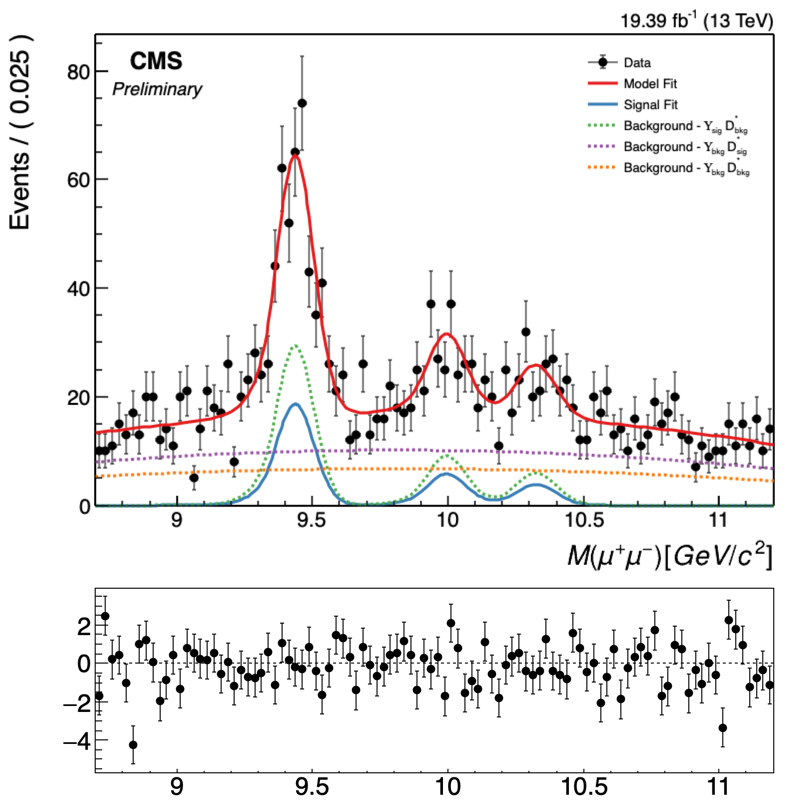
\includegraphics[width=0.23\textwidth]{figures/fit_rest/fit2D_upsilon_proj_2016APV.png}}}\hfill
    \subfloat[][2016 $\Upsilon$ projection.]{\label{subfig:fit2D_rest_upsilon_proj_2016}%
      \fbox{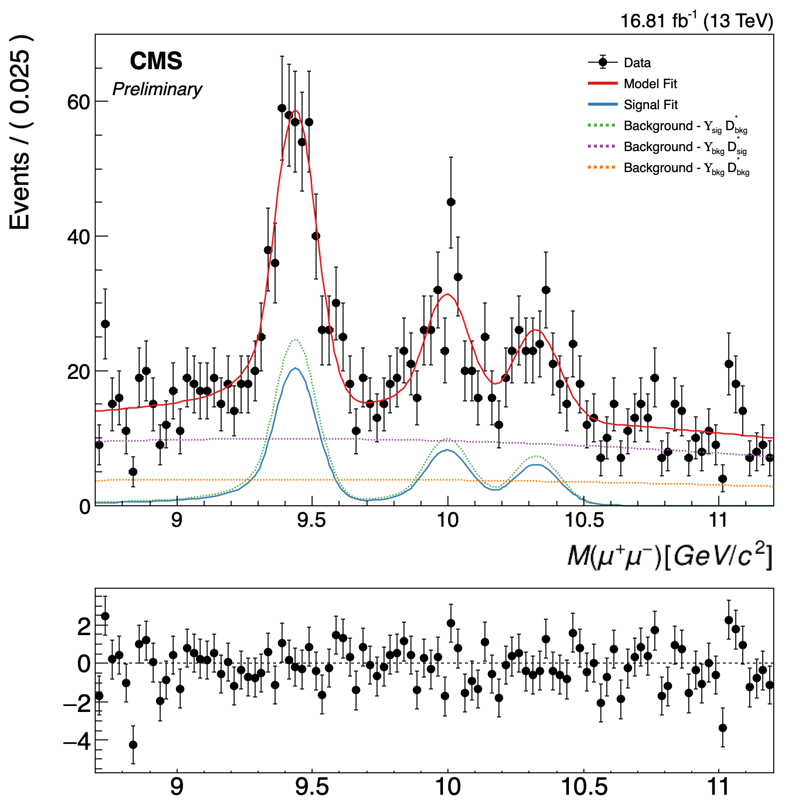
\includegraphics[width=0.23\textwidth]{figures/fit_rest/fit2D_upsilon_proj_2016.png}}}\hfill
    \subfloat[][2017 $\Upsilon$ projection.]{\label{subfig:fit2D_rest_upsilon_proj_2017}%
      \fbox{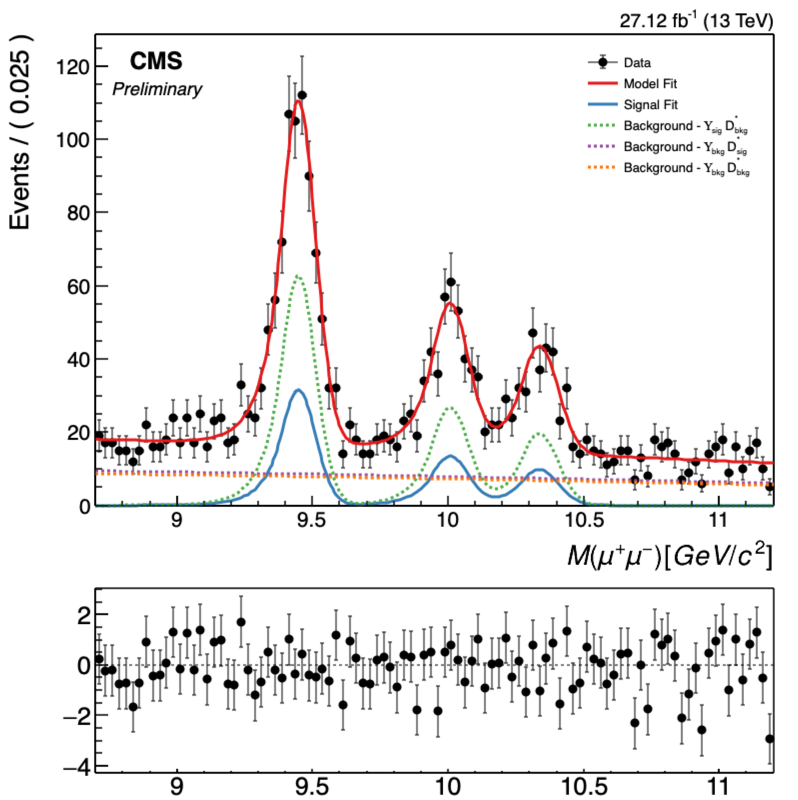
\includegraphics[width=0.23\textwidth]{figures/fit_rest/fit2D_upsilon_proj_2017.png}}}\hfill
    \subfloat[][2018 $\Upsilon$ projection.]{\label{subfig:fit2D_rest_upsilon_proj_2018}%
      \fbox{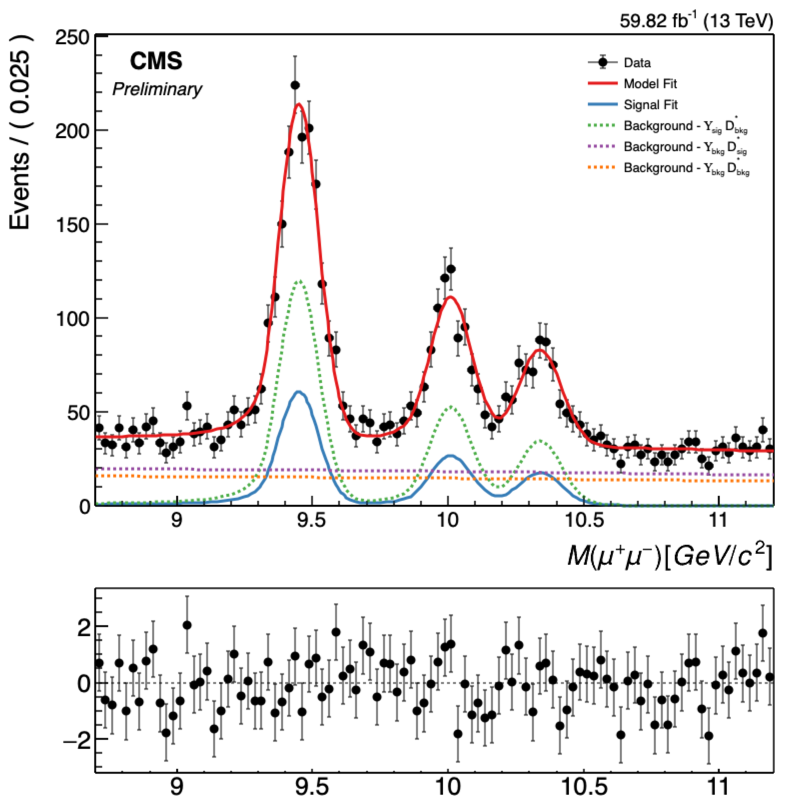
\includegraphics[width=0.23\textwidth]{figures/fit_rest/fit2D_upsilon_proj_2018.png}}}\\
    \subfloat[][2016APV D$^{*\pm}$ projection.]{\label{subfig:fit2D_rest_dstar_proj_2016APV}%
      \fbox{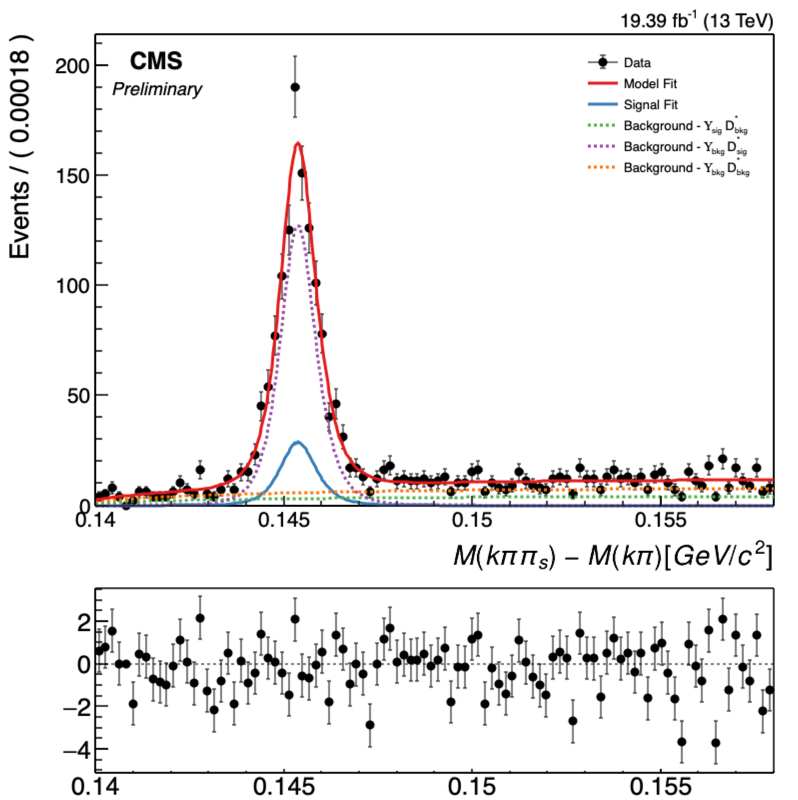
\includegraphics[width=0.23\textwidth]{figures/fit_rest/fit2D_dstar_proj_2016APV.png}}}\hfill
    \subfloat[][2016 D$^{*\pm}$ projection.]{\label{subfig:fit2D_rest_dstar_proj_2016}%
      \fbox{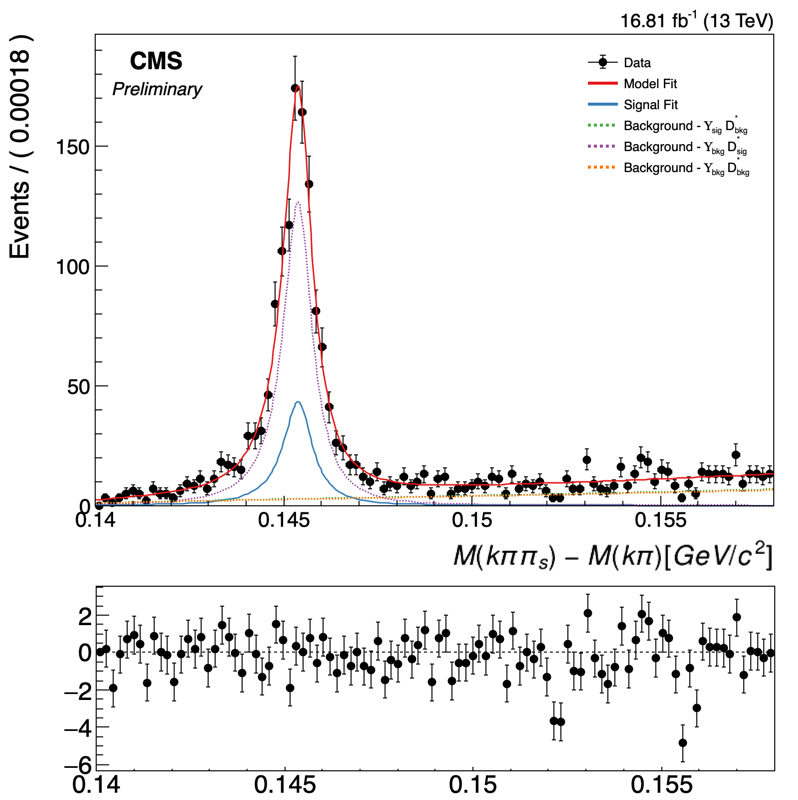
\includegraphics[width=0.23\textwidth]{figures/fit_rest/fit2D_dstar_proj_2016.png}}}\hfill
    \subfloat[][2017 D$^{*\pm}$ projection.]{\label{subfig:fit2D_rest_dstar_proj_2017}%
      \fbox{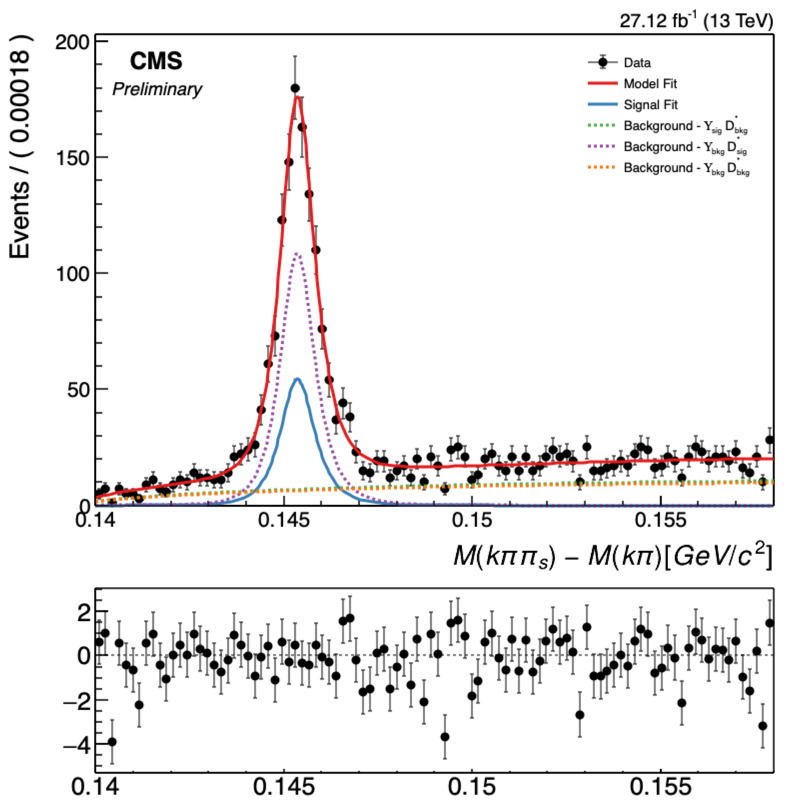
\includegraphics[width=0.23\textwidth]{figures/fit_rest/fit2D_dstar_proj_2017.png}}}\hfill
    \subfloat[][2018 D$^{*\pm}$ projection.]{\label{subfig:fit2D_rest_dstar_proj_2018}%
      \fbox{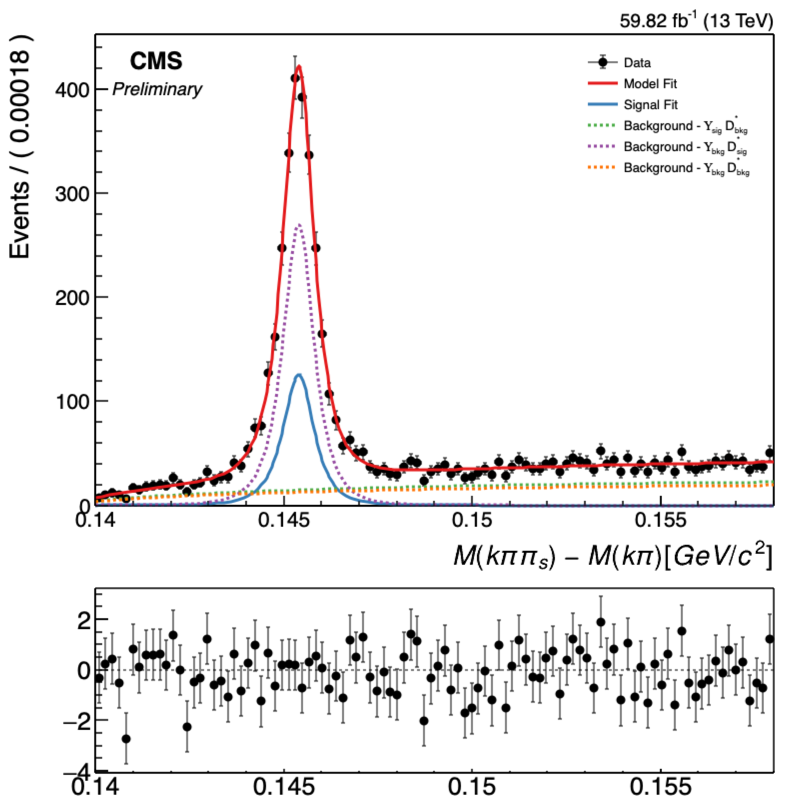
\includegraphics[width=0.23\textwidth]{figures/fit_rest/fit2D_dstar_proj_2018.png}}}\\
    \legend{Projections to the dimuon invariant mass (a-d) and D$^{*\pm}$ $\Delta$m (e-f) taken from the fit to the selected associated $\Upsilon + $ D$^{*\pm}$ for all data samples restricting the phase space to match the ones specified in Tab. \ref{tab:inclusive_xsec}. The curves represent the full fit (in red) and each of the components - signal in blue and continuous line and background components using dashed lines in green, purple and orange.}
  \end{figure}
\end{landscape}

\section{Systematic Uncertainties}

The systematic uncertainties include all the uncertainties that do not arise from the fluctuations in a finite set of measurements. This includes bias coming from the experiment, the assumptions made and models used to make the conclusions. The evaluation of this kind of uncertainty is analysis dependant, as one needs to consider all assumptions made in the measurement process.

That being said, the complete systematic uncertainty definition is not finished in this analysis due to time constraints, but some of them are brought in the following lines.

\begin{itemize}
  \item \textbf{Integrated Luminosity}: The integrated luminosity uncertainties are given in Refs. \cite{CMS-PAS-LUM-17-001, CMS-PAS-LUM-17-004, CMS-PAS-LUM-18-002} and are summarized in Tab. \ref{tab:triggers}. 
  \item \textbf{Branching Fraction}: The uncertainties on the branching fractions of each considered decay channel are given in Ref. \cite{Workman:2022ynf}. The values are pointed out in Sec. \ref{sec:theoryY+D}
  \item \textbf{Determination of the yields}: This systematic depends on the models used to determine the signal and background yields, in general, the models used to describe the shapes of the distributions. For D$^*$ signal, the model was changed to a double Gaussian and for the background another threshold function was used \cite{CMS:2021lab}, with the form
  \begin{equation}
    f = \left[ 1- \exp{\left( -\frac{\Delta m - m_\pi}{p_0} \right)} \right]\left( \frac{\Delta m}{m_\pi} \right)^{p_1} +p_2 \left( \frac
    {\Delta m}{m_\pi} - 1 \right),
  \end{equation}
  where $m_\pi$ is taken as the pion mass and $p_0$, $p_1$ and $p_2$ are free parameters. The deviations from the yields were taken as systematic uncertainties.

  For $\Upsilon$ signal, a change from CBs to Gaussians resulted to bad fits, as the later one cannot describe well the tails of the invariant mass distribution. Another method is to evaluate the CB shape changes with the change of its parameters. The tail parameters $n$ and $\alpha$ are specially sensitive as they are strongly correlated. $n$ was left as free parameter and $\alpha$ was moved by $\pm 2\sigma$. Half of the maximum observed variation was taken as systematic, because these variations are correlated. Another parameter analyzed was the mean of the CBs, which is defined from a common factor and the mass of the $\Upsilon$ state taken from Ref. \cite{Workman:2022ynf}. The means were left as a free parameter and the deviation in the yield is taken as a systematic.

  Finally, the $\Upsilon$ background model was modified to a 3rd order Chebychev polynomials and the deviation was taken as systematic.
  \item \textbf{Selection Cuts}: The selection cuts 
  \item \textbf{Tracking Efficiencies}: The tracking efficiency for charged hadrons is given by Ref. \cite{CMS-DP-2022-012}, using the branching ratios two D$^*$ decays: $D^* \rightarrow K\pi\pi_s$ and $D^* \rightarrow K3\pi\pi_s$. The uncertainty is given depending on the sample and it is combined for the two D$^0$ tracks. For $\pi_s$, a different procedure should be done, since it has a soft $p_T$ distribution. The value of 5.2 \%, given in Ref. \cite{CMS:2021lab} is used.
\end{itemize}